\documentclass[a4paper,11pt]{book}

\usepackage[left=2cm,right=2cm,top=2cm,bottom=2cm]{geometry}
\usepackage[utf8]{inputenc}
\usepackage[spanish,mexico]{babel}

\usepackage{amsmath, amssymb, amsthm}
%\usepackage{mathrsfs}
\usepackage{appendix}
\usepackage{bachelorstitlepageUNAM}
\usepackage{tikz-network}
\usepackage[linesnumbered,ruled,vlined]{algorithm2e}
\usepackage{minted}	
\usepackage{tcolorbox}
\usepackage{float}
%pdflatex -synctex=1 -interaction=nonstopmode --shell-escape %.tex



\usepackage{captdef}
\usepackage{psfrag}
\usepackage{graphicx}
%\usepackage{subfig}
\usepackage{color}
\usepackage{multicol} 
\usepackage{wrapfig}

\usepackage{cancel}
\usepackage[usenames,dvipsnames,svgnames,table]{xcolor}
\usepackage{caption}
\usepackage{subcaption}
%\usepackage{cite}
\renewcommand{\baselinestretch}{1.5}

\usepackage{hyperref}
%\usepackage[hidelinks]{hyperref} 
\hypersetup{
	colorlinks=true,
	linkcolor=blue,
	filecolor=magenta,      
	urlcolor=cyan,
}
\theoremstyle{plain}
\newtheorem{proposición}{Proposición}
\newtheorem{teorema}{Teorema}
\theoremstyle{definition}
\newtheorem{definición}{Definición}
\newtheorem{ejemplo}{Ejemplo}

\setcounter{tocdepth}{3}
\setcounter{secnumdepth}{3}
\usepackage{svg}

\begin{document}
	\thispagestyle{empty}
	
\includegraphics[height=3.5cm]{escudoCiencias.pdf}
	\vspace{-3.8cm}
	\begin{flushright}
		\hspace{4cm}
		{\Large\textbf{Análisis para $N=50$}\\
			Análisis de distribuciones estadísticas de la tesis}
		\vspace{0.3cm}\\
		\begin{large}Autor: Rodrigo Vega Vilchis.\end{large}\\
		\begin{footnotesize}
			\hspace{2.05cm}{\color{white}.}\\
		\end{footnotesize}
		\vspace{0.1cm}
		\begin{large} 
			Fecha: 19/05/25\end{large}\\
	\end{flushright}
	\vspace{.4cm}
	\hrule height1pt\vspace{.5cm}
	
\subsection{Análisis para $N=50$}

Como parte de la investigación, se tienen  a disposición un banco de \href{https://github.com/rogve98/Tesis/tree/master/Notebooks/Datos/Jacobianos}{Jacobianos} y otro de \href{https://github.com/rogve98/Tesis/tree/master/Notebooks/Datos/Diagonales}{Diagonales}\footnote{Para los Jacobianos acceder a: \url{https://github.com/rogve98/Tesis/tree/master/Notebooks/Datos/Jacobianos}. Para las Diagonales acceder a \url{https://github.com/rogve98/Tesis/tree/master/Notebooks/Datos/Diagonales}.} de Jacobianos en donde se concentran 78 archivos .csv en cada banco, y contienen cada uno la información de 100 simulaciones diferentes que resultaron ser estables. Debido al costo computacional, se tuvieron que generar para $N=50$ para los siguientes casos:
\begin{table}[h!]
	\centering
	\begin{tabular}{|c|c|c|c|}
		\hline
		Valor promedio [$\sigma$] & Probabilidades [$p$] & Cantidad de archivos & Simulaciones realizadas \\ \hline
		$0.1-0.5$  & $0.1-1.0$  & 50 & 5000  \\ \hline
		0.6  & $0.1-0.9$  & 9 & 900 \\ \hline
		0.7  & $0.1-0.7$  & 7 & 700 \\ \hline
		0.8  & $0.1-0.5$  & 5 & 500 \\ \hline
		0.9  & $0.1-0.4$  & 4 & 400 \\ \hline
		1.0  & $0.1-0.3$  & 3 & 300 \\ \hline
		& \textbf{Total:} & 78& 7800\\ \hline
	\end{tabular}
	\caption{Cantidad de archivos generados para el banco de Diagonales y Jacobianos considerando $N=50$. A partir de $\sigma=0.6$ en adelante, los tiempos de compilación fueron muy prolongados por lo que no se obtuvieron los 10 archivos respectivos a diferencia de los valores promedio anteriores.}
	\label{tab:Simulaciones}
\end{table} 

La razón de explorar sistemas estables para valores de $\sigma$ y $p$ cercanos a 1.0 era para ver que tan probable era que fueran estables en estas condiciones, además de obtener un mínimo de información posible para fortalecer el análisis que se hará a continuación. Se busca realizar una caracterización de las distribuciones enfocándose principalmente en la relación que tiene la media con la desviación estándar de cada una de las 7800 distribuciones; sobre todo ver de que forma cambia en función de los parámetros $\sigma$ y $p$. Con base en los resultados encontrados, se explorará si también existe una relación entre la distribución de las diagonales con la distribución de la parte real de los eigenvalores asociados a los sistemas estables, de esta forma se podrá justificar parcialmente la propuesta de las \textit{Leyes Circulares}, que indica que cada valor de la diagonal puede fungir como centro y radio de una de $N$ leyes circulares que encierran localmente cierta cantidad de eigenvalores del sistema.

\subsubsection*{Diagonales}

Algo que se ha visualizado en un primer acercamiento (Figura (\ref{fig:DistDiagonal})) es que cuando es más grande la conectividad del sistema (parámetro $p$), la distribución de la diagonal es más amplia. Se confirmará esto con los datos disponibles y además se verá si ocurre algo similar para $\sigma$ en las mismas circunstancias. A continuación se revisará de forma cualitativa la forma de algunas distribuciones de diagonales asociadas a ciertas $p$ y $\sigma$ con $N=50$
\begin{figure}[h!]
	\centering
	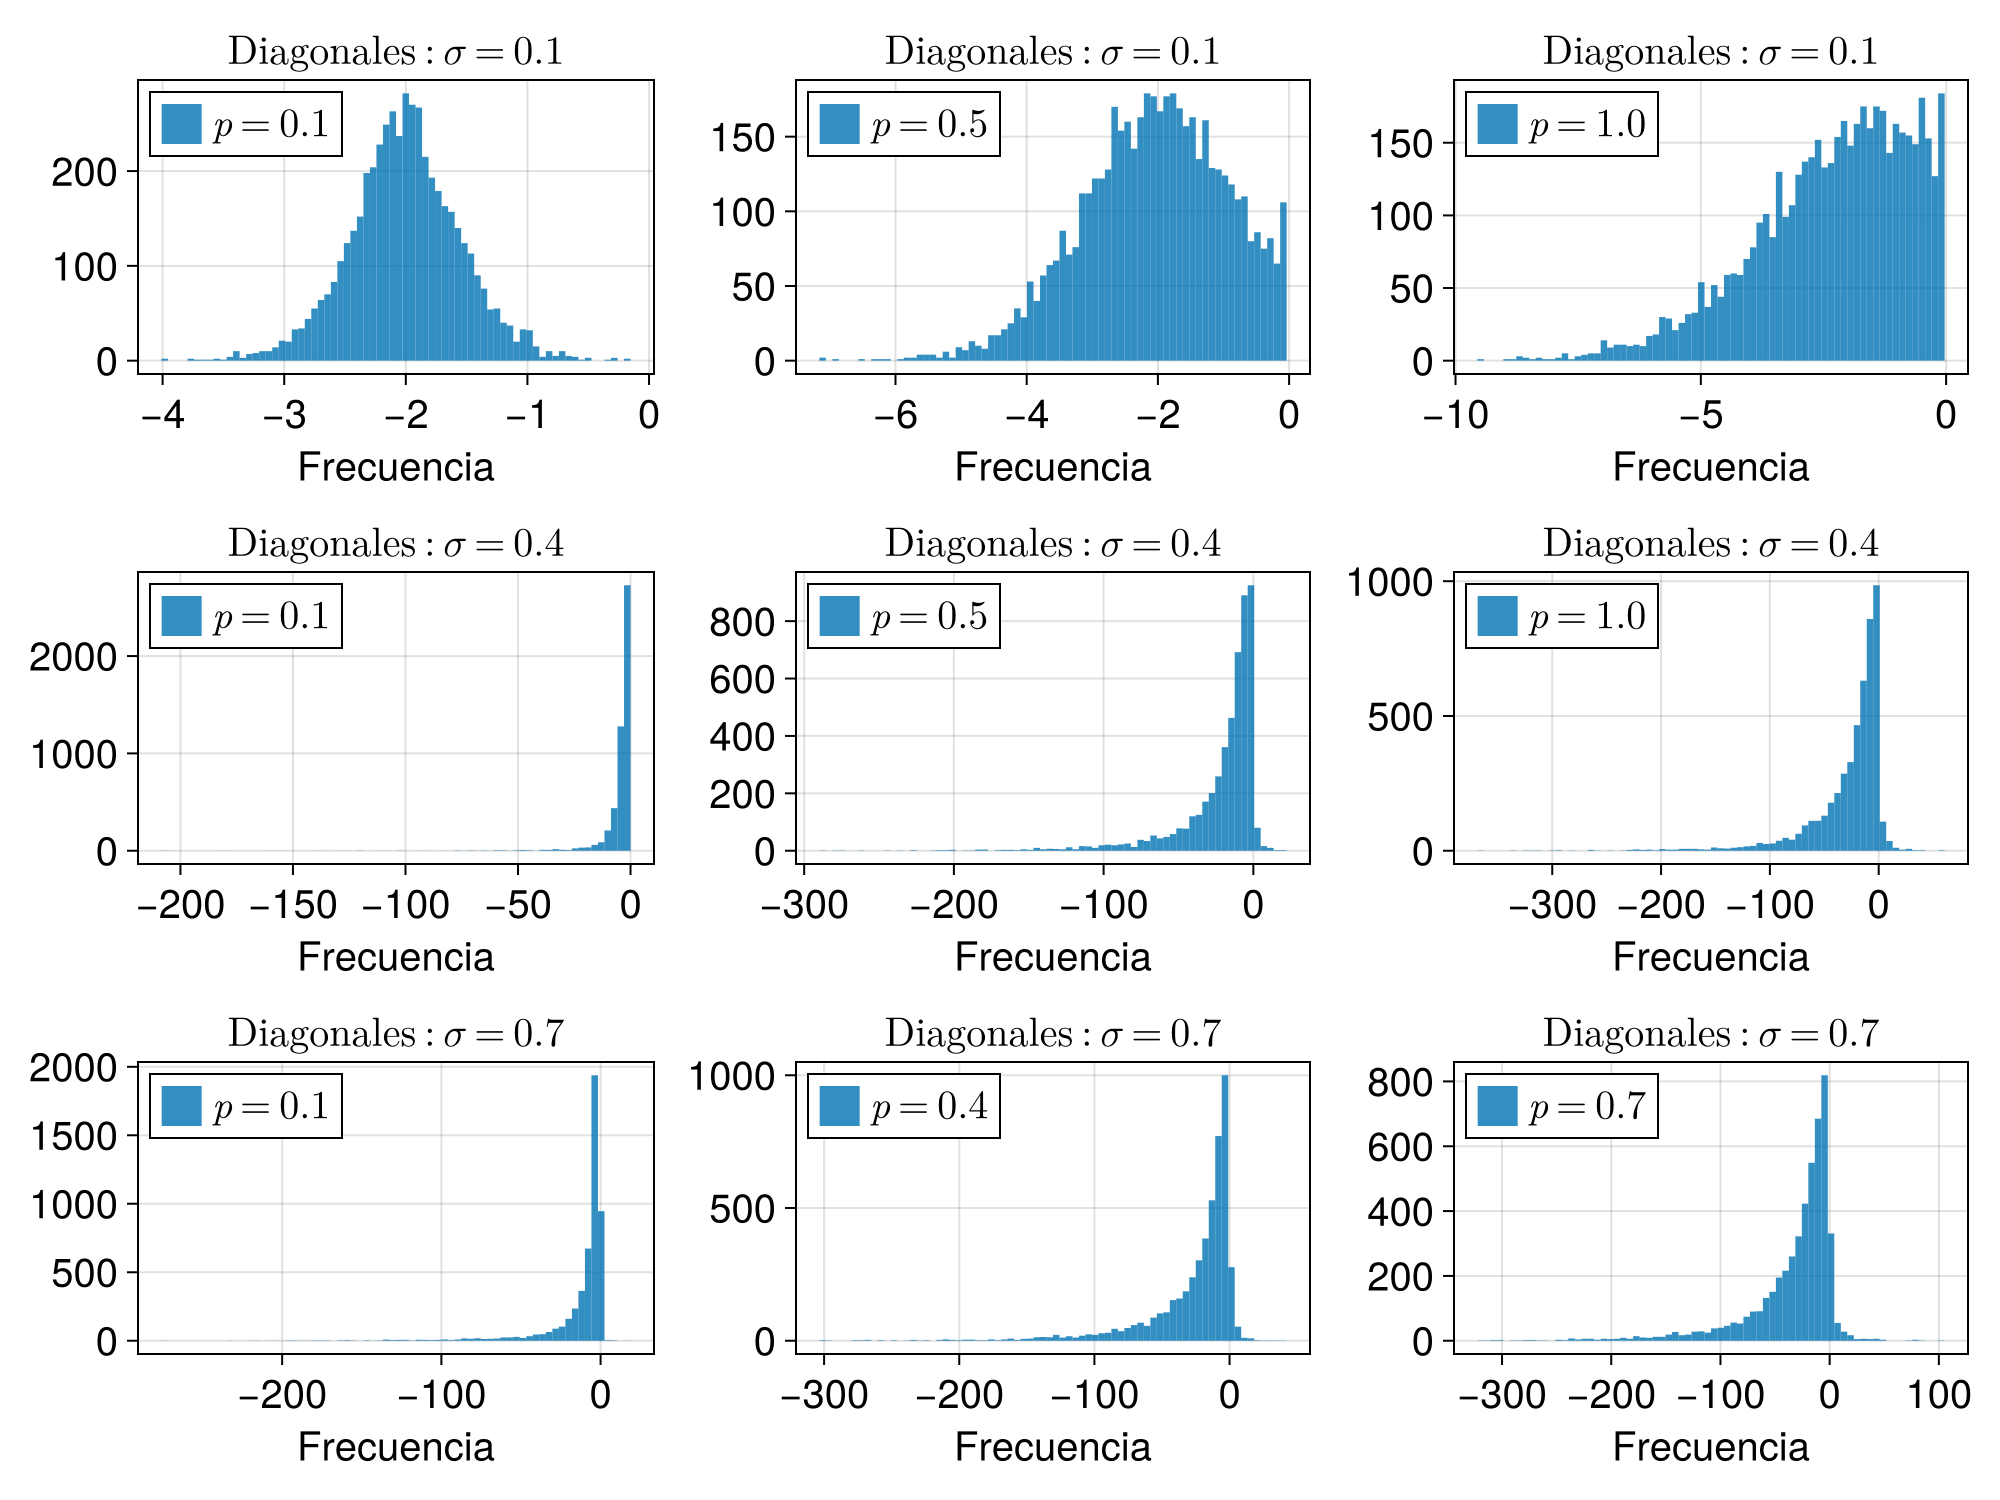
\includegraphics[scale=0.24]{../Imagenes/distDiagonales50}
	\caption{Distribución de 500 diagonales resultantes de 100 sistemas estables/cuasi-estables para $N=50$. Cuando $\sigma$ y $p$ tienden hacia 1, aumenta la tendencia hacia distribuciones de cola pesada.}
	\label{fig:distDiagonales50}
\end{figure}

Se puede observar que la distribución de las diagonales tiene una tendencia FDP normal para los casos con $\sigma=0.1$, sin embargo conforme las probabilidades aumentan, haciendo que los sistemas sean cada vez más conectados, la distribución se va ensanchando y sesgando hacia la izquierda. Para los casos $\sigma=0.2$ en adelante, se sigue una tendencia de distribución de cola pesada. Las distribuciones al no ser simétricas, indican que la media estadística $\langle d_{kk}(\sigma_i,p_j)\rangle$ se encuentra hacia la izquierda de la moda estadística. Para cada $\sigma$ se observa que a medida que $p$ aumenta, la distribución se ensancha siendo cada vez más dispersa; por lo tanto la media estadística se va desplazando hacia la parte negativa a medida que la desviación estándar $s(d_{kk}(\sigma_i,p_j))$ es más grande.
\\
\\
Cuando se observa que las distribuciones son más compactas, entonces la media puede encontrarse en un valor más cercano al cero. Esto puede indicar que existe una correlación entre ambas medidas estadísticas por lo que se tendría que comprobar este hecho. La forma de la distribución de las diagonales puede asemejarse a la distribución Log-Normal que es bien conocido que tiene una relación no trivial entre su media y desviación estándar [cita\footnote{Cita}], sin embargo, al realizar los ajustes correspondientes, se encuentra que el $p$-valor es suficientemente cercano a cero como para descartar esta hipótesis. \\
\\
Debido a ello solamente se asumirá que es una distribución con sesgo negativo. Se ha determinado un ajuste lineal ``general'' para las 7800 simulaciones únicamente para notar si el comportamiento es 
\begin{wrapfigure}{r}{0.5 \textwidth} \vspace{-20pt} \begin{center}
		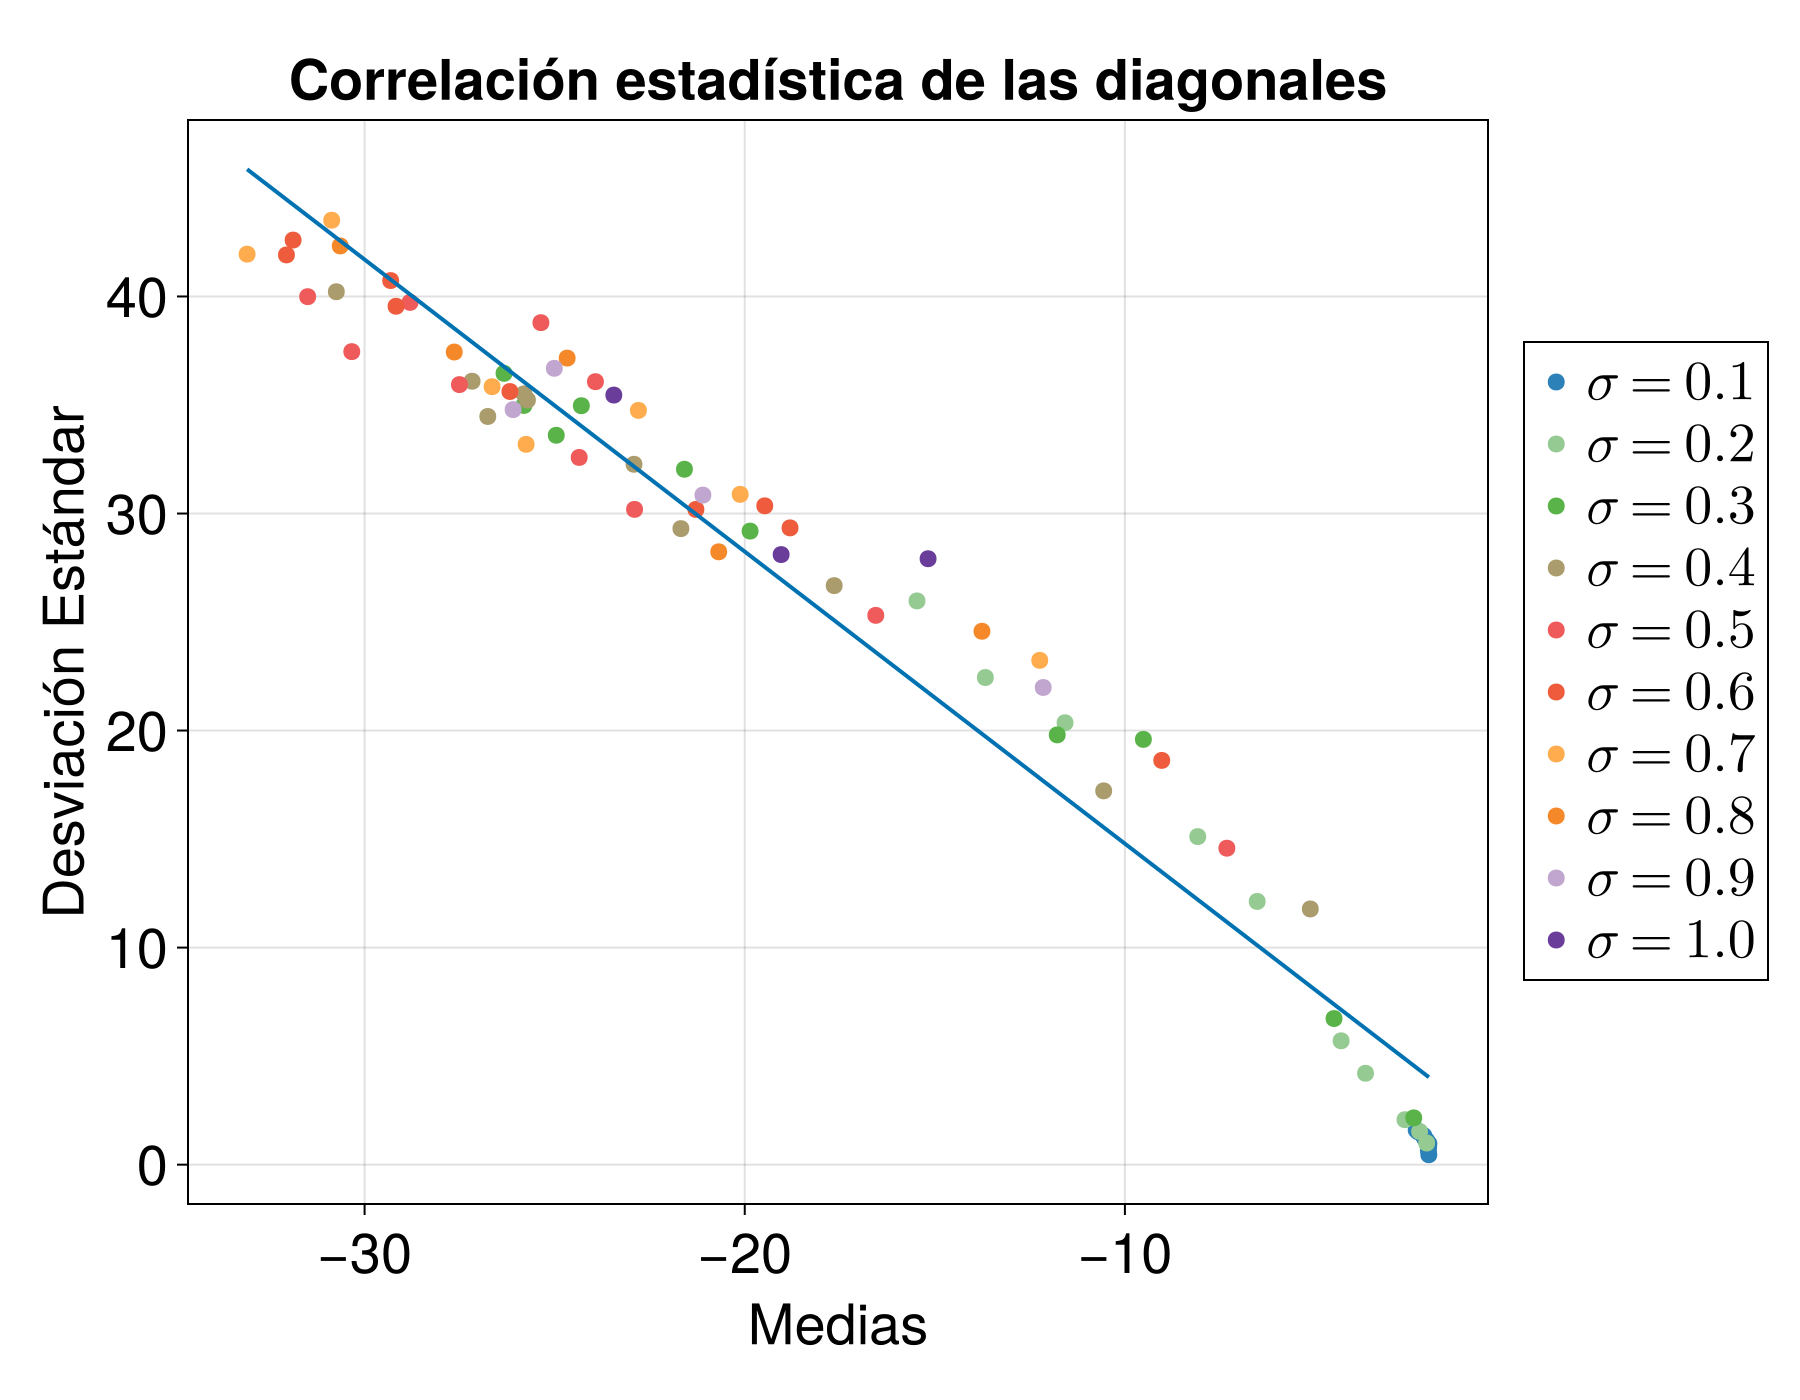
\includegraphics[scale=0.15]{../Imagenes/CorrelacionMvsStd}
	\end{center}
	\vspace{-20pt} 
	\caption{Ajuste lineal entre los promedios y las desviaciones estándar de cada una de las 7800 simulaciones realizadas bajo los parámetros que dicta la Tabla (\ref{tab:Simulaciones}).}
	\vspace{-10pt}
	\label{fig:CorrelacionMvsStd}
\end{wrapfigure}
compartido entre diferentes parámetros de $\sigma$ y $p$. Cada color corresponde con una $\sigma$ definida y las probabilidades se distinguen a partir de la media/desviación estándar, entre más grande sea el valor de $p$ también será más grande la magnitud de las anteriores. El comportamiento general es que existe una relación lineal entre la media y la desviación estándar. Cuanto más grandes son $\sigma$ y $p$, la media se desplaza hacia los valores negativos y las distribuciones son cada vez más dispersas.
Habría de ejecutarse un ajuste lineal para cada $\sigma$, sin embargo, con los datos disponibles se puede determinar los coeficientes de correlación para cada $\sigma$ y corroborar de manera indirecta lo que nos anuncia la gráfica (Tabla (\ref{tab:Correlaciones})). Lo que se puede observar es que se tiene una muy fuerte correlación entre ambas cantidades estadísticas, a excepción de los casos $\sigma=\{0.1,1.0\}$ en donde se tienen los coeficientes bajos. \\
\\
El primer caso es muy especial ya que las observaciones indican que las distribuciones de diagonales pasan de ser simétricas (normal) a ser una distribuciones con sesgo negativo a medida que $p$ vaya aumentando. Realizando un ajuste lineal al caso $\sigma=0.1$ se podrá ver que no es tan bueno como en el resto de los casos, muy posiblemente se deba a esta evolución hacia las distribuciones con sesgo negativo. Para el segundo caso simplemente haría falta más información para poder comprobar si en verdad es fuerte o débil la correlación\footnote{Aún así con las 300 simulaciones para $p=\{0.1,0.2,0.3\}$ la correlación es considerablemente fuerte, aunque no tanto como en el resto de los casos.}. Lo mismo ocurre para los conjuntos de simulaciones $\sigma=\{0.6,0.7,0.8,0.9\}$, le hacen falta información para todos aquellos casos (probabilidades) que por cuestiones de complejidad del sistema y demanda computacional no se pudieron concretar; pero aún con la información disponible indican una muy fuerte correlación entre las medidas estadísticas y las desviaciones estándar consideradas. 
\begin{table}[h!]
	\centering
	\begin{tabular}{|c|c|}
		\hline
		Fuerza de interacción promedio: $\sigma$ & corr($\langle d_{kk}(\sigma_i,p_j)\rangle,s(d_{kk}(\sigma_i,p_j)))$ \\ \hline
		0.1 & -0.8798 \\ \hline
		0.2 & -0.9920\\ \hline
		0.3 & -0.9829 \\ \hline
		0.4 & -0.9963\\ \hline
		0.5 & -0.9630 \\ \hline
		0.6 & -0.9954 \\ \hline
		0.7 & -0.9646 \\ \hline
		0.8 & -0.9675 \\ \hline
		0.9 & -0.9818 \\ \hline
		1.0 & -0.8943 \\ \hline
	\end{tabular}
	\caption{Correlación entre la media ($\langle d_{kk}(\sigma_i,p_j)\rangle$) y la desviación estándar ($s(d_{kk}(\sigma_i,p_j))$) de cada una de las 7800 simulaciones. Se considera por cada conjunto de $\sigma_i$ para toda $p_j$ disponible según la Tabla (\ref{tab:Simulaciones}).}
	\label{tab:Correlaciones}
\end{table} 

La máxima correlación se visualiza en la región dada por el conjunto $\sigma=\{0.2,0.3,0.4,0.5,0.6\}$, misma en donde los sistemas suelen ser estables con una alta probabilidad. Aún así en cada caso, pueden existir algunas variaciones en la forma de dispersión de las distribuciones consideradas, las cuales se pueden medir a través del \textit{Coeficiente de variación} definido como
\begin{equation}\label{eqn:CV}
	CV=\frac{s(d_{kk}(\sigma_i,p_j))}{|\langle d_{kk}(\sigma_i,p_j)\rangle|}
\end{equation}
El coeficiente indica que si tiene valor $CV=1$, la media y la dispersión se encuentran equilibradas, mientras que para $CV<1$ la dispersión es menor a la media y en caso contrario la dispersión es mayor a la media. Este coeficiente solamente relaciona las cantidades anteriores, no habla de que tan ancha es la distribución tal y como se mostró en la Figura (\ref{fig:CorrelacionMvsStd}). Servirá para ubicar cómo es la dispersión de la distribución para cada caso $d_{kk}(\sigma_i,p_j)$ y como evoluciona en función de $\sigma$ y $p$.
\newpage
\begin{table}[h!]
	\centering
	\begin{tabular}{|c|c|c|}
		\hline
		Coeficiente de variación promedio $\langle CV\rangle$ & $\min(CV)$ & $\max(CV)$ \\ \hline
		1.3354 & 0.2280 & 2.2995\\ \hline
	\end{tabular}
	\caption{Se determinan los 78 coeficientes de variación disponibles según la Tabla (\ref{tab:Simulaciones}) y se determina el promedio, mínimo y el máximo del conjunto total.}
	\label{tab:CVs}
\end{table} 
Una vez determinando los 78 coeficientes de variación se puede observar que en promedio las desviaciones estándar son mayores a las medias de las distribuciones $d_{kk}(\sigma_i,p_j)$, lo que indica que en general las distribuciones son dispersas y sustentan el carácter de cola pesada: se confirma de manera directa lo que se ha estado discutiendo con anterioridad. Con el mínimo y el máximo del conjunto de coeficientes se establece un rango que nos da una idea de que tan dispersas son las distribuciones, anuncia que existen más distribuciones con desviación estándar mayor a la media que en su caso contrario. Para corroborarlo es necesario graficar las variaciones del conjunto de coeficientes de variación:
\begin{figure}[h!]
	\centering
	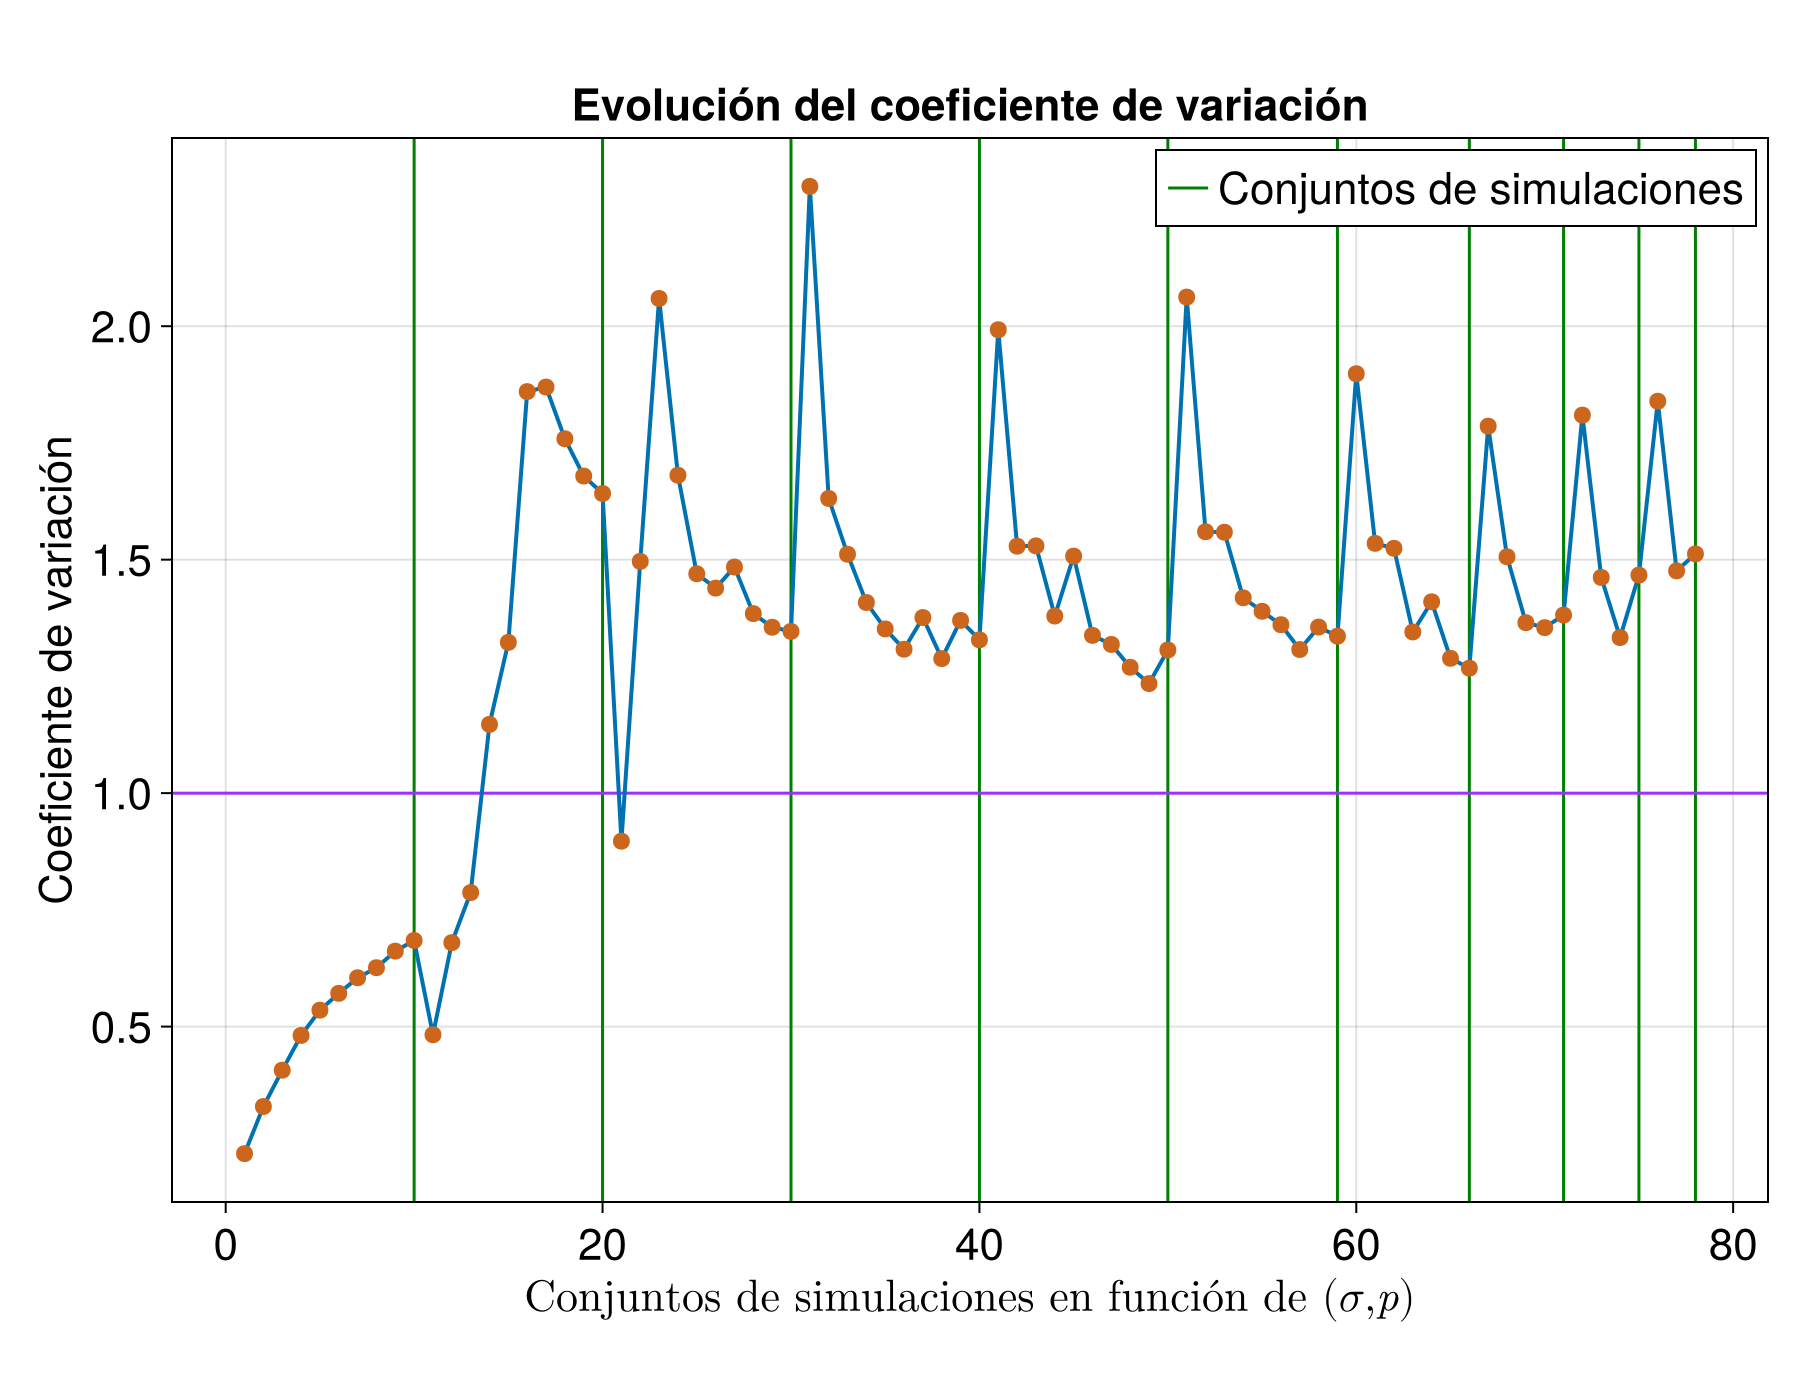
\includegraphics[scale=0.24]{../Imagenes/CoeficientesVariacion}
	\caption{Evolución del coeficiente de vaiación en función de $\sigma$ y $p$. Cada coeficiente se muestra para un conjunto de simulaciones dependientes de $\sigma_i$ y $p_j$ según la Tabla (\ref{tab:Simulaciones}).}
	\label{fig:CoeficientesVariacion}
\end{figure}

Del gráfico se pueden analizar varios puntos: para el conjunto de datos $\sigma=0.1$ se observa que la desviación estándar es menor al valor de sus medias, lo que indica que no son distribuciones muy dispersas o de cola pesada tal y como sucede con el resto de las distribuciones, además de que se ha observado que se comienza en una FDP normal que se va sesgando hacia la izquierda conforme $p$ aumenta. Esto se puede apreciar desde el esbozo de la Figura (\ref{fig:distDiagonales50}). Además del sesgo, si se encuentra bien marcada la tendencia de que la dispersión aumente conforme $p$ también lo haga. Ocurre algo interesante para $\sigma=0.2$, comienza con baja dispersión con respecto de la media y para $p\geq0.4$ emergen las distribuciones con alta dispersión. En este caso también se observa una ligera transición entre una FDP normal truncada que se va sesgando hacia la izquierda, sin embargo el resto de conjuntos de $\sigma$ las distribuciones comienzan sesgadas hacia la izquierda con cola pesada.\\
\\
A partir de $\sigma=0.3$ en adelante se puede observar un patrón interesante, se tiene un punto máximo del coeficiente de variación que indica una máxima dispersión y después disminuye, como si la cola pesada se suavizara. Y justamente eso es lo que ocurre, para cada $\sigma\geq 0.3$ con $p=0.1$, un gran porcentaje de la distribución se concentra cerca de la media mientras que son muy pocos los valores que se encuentran en la cola pesada. Conforme $p$ vaya aumentando en estos escenarios, la desviación estándar va disminuyendo con respecto de la media lo que indica que la distribución es cada vez menos dispersa haciendo que a su vez existan más valores que se concentren en la cola pesada. ¡Y esto ocurre similarmente para cada $\sigma\geq 0.3$!\\
\\
Algo importante de preguntarse es ¿por qué en general las distribuciones son de cola pesada con sesgo negativo? todo viene a raíz de como se definió la matriz de interacciones (Definición \ref{def:MatrizInteracciones}) y a su vez de como está construida la matriz de incidencias (Definición \ref{def:MatrizIncidencias}). Es fácil responder la parte del signo, desde un principio las diagonales siempre fueron negativas y se encuentra sustentado en la Proposición \ref{prop:DiagonalI}, por lo que las distribuciones siempre tuvieron que ser negativas\footnote{Aunque si se observa en la \ref{fig:distDiagonales50} se puede ver como para $\sigma$ y $p$ altas, las distribuciones tienen valores positivos; esto podría no ser congruente con la Proposición \ref{prop:DiagonalI} y más adelante se discutirá lo que ocurrió aquí.} pero con el carácter de cola pesada y además sesgada se tendrá que desarrollar un argumento más fuerte.\\
\\
Aunque estas distribuciones no tengan relación con FDP Log-Normales, es posible rescatar algunos elementos de su construcción para argumentar nuestra conjetura actual. Es bien conocido que para una variable aleatoria: si sus cambios son multiplicativos entonces se genera una distribución de cola pesada [cita\footnote{Para una variable aleatoria $X$, si el proceso multiplicativo es $X_t=X_{t-1}\cdot e	^{\epsilon_t}$, donde $\epsilon_t\sim \mathcal{N}(\mu,\sigma^2)$.}]. Además de ello, los mismos factores multiplicativos son los que determinan el sesgo de la distribución, en nuestro caso particular: de carácter negativo. Recordar que los valores de la diagonal vienen determinados por

$$\mathcal{I}_{ii} = r_i \left (1-\frac{2x_i+\sum_{j\neq i}\alpha_{ij}x_j}{K_i}\right ),\qquad\text{para }i\in\{1,...,N\}$$
\newpage
Claramente el término de la tasa de crecimiento $r_i$ reescala a todo $\mathcal{I}_{ii}$ de modo que las fluctuaciones que se generen con base en $x_i$ y $x_j$ se magnifican en función de esta $r_i$. No obstante, el valor intrínseco del término de la diagonal viene bien dictada por la relación de estas $x_i$ y $\alpha_{ij}x_j$ divididos por $K_i$\footnote{Donde las $x_j$ y $x_i$ son las entradas del atractor del sistema.}, donde se sabe que estos coeficientes vienen de una distribución normal centrada en $\mu=0$ con las $\sigma$s que se han venido considerando hasta ahora. Por lo tanto bien pueden existir valores extremos que se ubiquen en la cola pesada como puede haber valores que se concentren entorno a una media ($\langle d_{kk}(\sigma_i,p_j)\rangle$, Ver Figura (\ref{fig:TrMedStd}, \textbf{B})) dependiendo totalmente de como se encuentren configuradas las $\alpha_{ij}x_j$ que como recordatorio: vienen de la \textit{red de incidencias}. \\
\\
El motivo del sesgo se deberá a que son más comunes los coeficientes de interacción $\alpha_{ij}$ de la distribución normal entorno a $\mu=0$ con su respectiva $\sigma$ en comparación con los que se encuentren en los extremos de la misma, en especial cuando se tienen pocas interacciones ($p$ baja). Por lo tanto las sumas y el re-escalamiento de $\mathcal{I}_{ii}$ se concentra entorno a cierta moda estadística y en concreto	se ajusta en torno a $2$ que coincide con el valor fijo que se le dio al parámetro $r_i$. Cuando se tienen mayor número de 
\begin{wrapfigure}{l}{0.5 \textwidth} \vspace{-30pt} \begin{center}
		\includegraphics[scale=0.135]{../Imagenes/ModasEstadísticas}
	\end{center}
	\vspace{-20pt} 
	\caption{Modas de las distribuciones de diagonales disponibles dadas por la Tabla (\ref{tab:Simulaciones}).}
	\vspace{-10pt}
	\label{fig:ModasEstadísticas}
\end{wrapfigure}
interacciones ($p$ alta) es más probable que aumente la cantidad de valores extremos de las $\alpha_{ij}$ asociadas a $\mathcal{N}(\mu=0,\sigma)$ y en consecuencia la suma y los reescalamientos pueden situarse en valores más allá del 2 tal y como se puede apreciar en la Figura (\ref{fig:ModasEstadísticas}). Esta causa es la clave para que la media $\langle d_{kk}(\sigma_i,p_j)\rangle$, la desviación estándar $s(\sigma_i,p_j)$ y la moda estadística de las distribuciones de valores de las diagonales de los sistemas \textbf{estables} se vaya desplazando cada vez más hacia los valores negativos conforme $\sigma$ y $p$ aumenten: la estructura multiplicativa subyacente de la diagonal de la matriz de interacciones y las fluctuaciones que producen $x_i$ en conjunto con las $\alpha_{ij}x_j$ divididos por $K_i$ son la causa de este comportamiento. Para verificar si verdaderamente se trata de una propiedad de los sistemas estables, se habrían de generar más experimentos para otras $r_i$ y $K_i$ y validar si es reproducible este comportamiento. 

\subsubsection*{Relación con la estabilidad y eigenvalores de los sistemas.}

¿Qué relación tienen las diagonales con la estabilidad del sistema? Una fuerte hipótesis se puede realizar a partir de ello, pues resulta que de todos los sistemas que resultaron estables (salvo unas excepciones), tienen a sus diagonales con sus elementos negativos, sugiriendo que la diagonal es una fuerte componente decisiva para volver a los sistemas estables. No existe por ahora un teorema que resuelva esta conjetura, pues deben existir contra ejemplos en donde los elementos de la diagonales son negativos pero el resto de entradas de la matriz impacta de tal modo que vuelve al sistema inestable. Por ahora las simulaciones sustentan el argumento de la estabilidad pero entonces ¿qué pasa con las diagonales que resultaron positivas?  respectivamente) ¿impactarán también en la distribución de eigenvalores con algunos de ellos con parte real positiva? ¿Con base en el procedimiento, como es que se llegó a estos escenarios? (Ver Figura (\ref{fig:distDiagonales50}) para $\sigma=\{0.4,0.7\}$ con $p=\{1.0,0.7\}$)\\
\\
Como el mecanismo para determinar que los sistemas fueran estables o no se hizo a partir de revisar que las series de tiempo no divergieran, ha sucedido que para $\sigma$ y $p$ cercanos a 1.0, los sistemas tienen mayor dificultad para estabilizarse por la cantidad de interacciones existentes, a su vez las fluctuaciones que se producen provocan el retardo  de la estabilización. Lo ideal hubiera sido prolongar el tiempo de integración a $t_f=100$ para estos casos y verificar si suceden dos cosas: o logran llegar al atractor o también es posible lleguen a un punto crítico inestable haciendo que divergan las soluciones tras un efecto de retardo igualmente. \\
\\
Por lo tanto, debido al tiempo de integración: las series de tiempo se han quedado a medias para resolver en alguno de los dos escenarios anteriores. Esto es importante ya que se ha tomado el último punto de la serie como aquel vector $N$-dimensional considerado para evaluar en la matriz jacobiana que da origen a la matriz de interacciones. En conclusión existe un cierto número de matrices de interacción con esta situación y que por lo tanto no son estrictamente matrices de interacción, pues no  se encuentran evaluadas sobre un punto crítico. Sin embargo se ha intentado realizar una técnica para poder intentar llegar a ese posible atractor: consiste en utilizar el método de Newton-Rhapson multivariado para hallar el punto crítico que se espera.\\
\\
Se utilizaría como condición inicial el último punto de la serie de tiempo ya que se esperaría que el atractor estuviera cerca de esa región y se llegaron a dos resultados principales: Si la matriz resultante tiene de 1 a 3 entradas positivas, es probable que si encuentre el atractor y entonces terminemos de concluir que si se trataba de un sistema estable. El segundo resultado es menos esperanzador, pues si se tienen más de 3 entradas positivas, aún ejecutando Newton-Rhapson multivariado con las condiciones mencionadas, el algoritmo no devuelve al punto crítico atractor: de aquí se desprenden dos posibles escenarios, el primero y más directo es simplemente asumir que el sistema no era estable y que tuvo una acción retardada para que las soluciones divergieran. El segundo escenario es que debido a la condición inicial propuesta, el algoritmo solamente pudo aproximarse a un punto silla que se encontraba más próximo que el atractor y que gracias a ello no sea posible acceder a este segundo punto crítico que es el que se espera.\\
\\
No es trivial encontrar puntos críticos para sistemas $N\gg1$ aún teniendo métodos numéricos que ayuden a simplificar la tarea, pues se sabe que existen más de $N$ en cuestión y no se sabe con exactitud en que región del hiper-espacio se encuentra al menos uno de ellos que es el atractor. Por lo que se concluye esta parte con el hecho de que no hay forma de saber con la información actual que tipo de estabilidad tenían, la alternativa sería repetir esos experimentos considerando un tiempo de integración mayor a $50$ esperando que lleguen a su respectivo atractor.\\
\\
Excluyendo por ahora los casos de las diagonales con entradas positivas, ¿cual es la relación de las diagonales negativas con respecto de la estabilidad de los sistemas? Se puede plantear que mientras las trazas de las matrices sean negativas el sistema es estable, pero en esto hay que poner una restricción: las trazas negativas con todos lo valores de la diagonal negativos. Si existe al menos un valor positivo en la diagonal del Jacobiano del sistema, entonces cabe la posibilidad de que exista al menos un eigenvalor positivo que volvería intestable al sistema. Los experimentos han mostrado que la diagonal es un factor determinante para la estabilidad de estos sistemas, aunque no es absoluto si es un requisito importante que debe cumplirse. Las trazas de las matrices guardan una íntima relación con las medias ($d_{kk}(\langle \sigma_i,p_j)\rangle$) y a su vez como ya se ha visto anteriormente, con la desviación estándar $s(\sigma_i,p_j)$
\begin{figure}[h!]
	\centering
	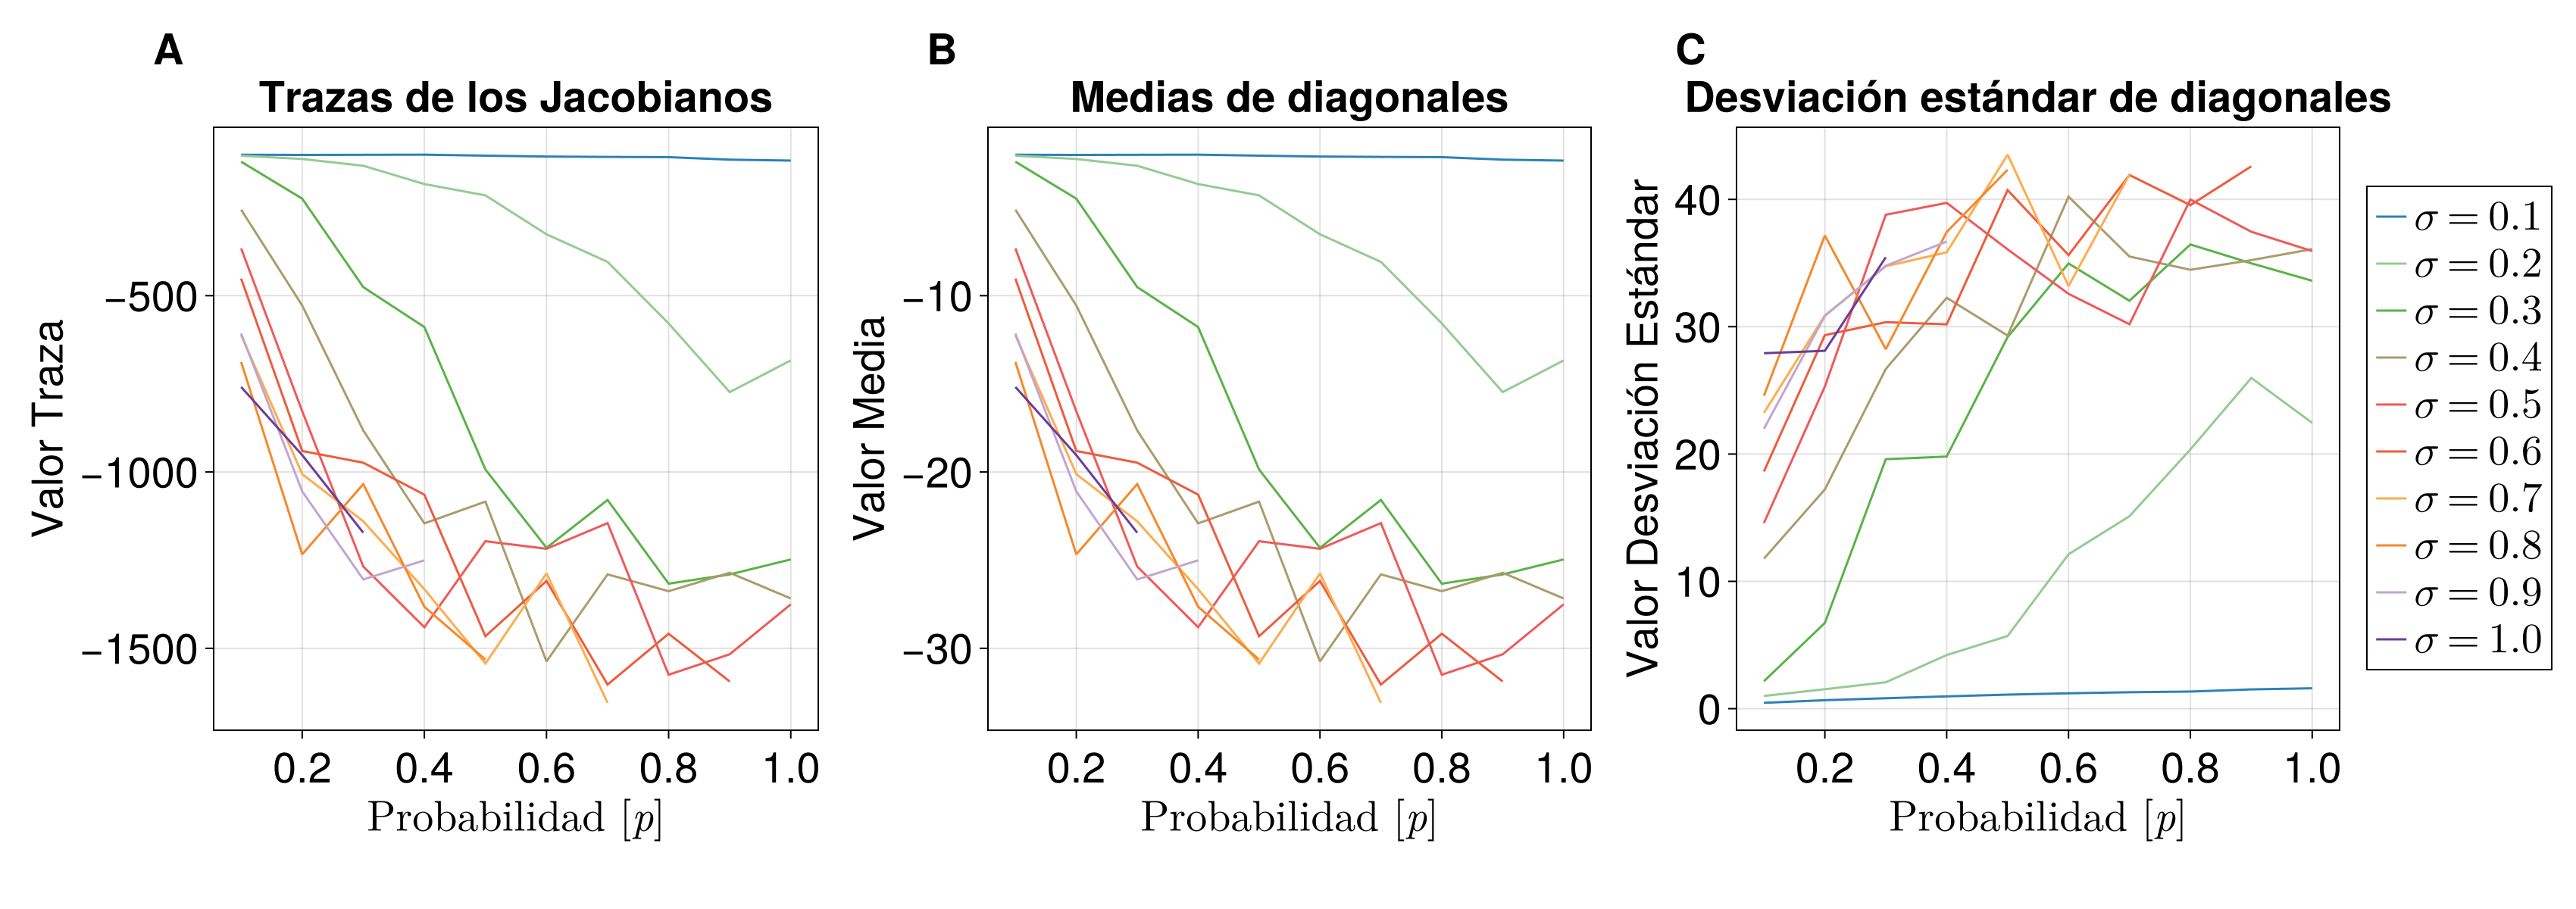
\includegraphics[scale=0.15]{../Imagenes/TrMedStd}
	\caption{Cada una de las cantidades se considera con base en las simulaciones disponibles. (\textbf{A}) Evolución de las trazas de los jacobianos del sistema. (\textbf{B}) Evolución de las medias de las diagonales de los jacobianos del sistema. (\textbf{C}) Evolución de la desviación estándar de las diagonales de los jacobianos del sistema.}
	\label{fig:TrMedStd}
\end{figure}

Aquí se puede ver de manera directa la relación que aparece retratada en la Figura (\ref{fig:CorrelacionMvsStd}), a medida que la traza/media de las simulaciones disminuye hacia valores cada vez más negativos, la desviación estándar por el contrario va aumentando. ¿Cuál será la relación de las diagonales de los jacobianos con respecto de su distribución de eigenvalores?

\subsubsection*{Distribución de valores propios}

Anteriormente se había propuesto, con un argumento cualitativo de la Figura (\ref{fig:LeyesCirculares}), que existen $N$ \textit{leyes circulares} donde a cada una de ellas le corresponde un centro y radio de cada valor de la diagonal del jacobiano del sistema. De esta manera cada ley circular encierra cierta cantidad de valores propios del sistema. Con la información provista de las simulaciones realizadas, se puede determinar un argumento estadístico más fuerte para sostener esta propuesta. \\
\\
La clave estará en revisar si existe una correlación estadística entre los valores de las diagonales mencionadas con las partes reales de los eigenvalores, se ha observado que para algunas simulaciones la relación fue casi perfecta mientras que para otras no tanto. Lo interesante de ver es que la relación es mejor cuando el valor de $p$ es alto, es decir, cuando hay cada vez más interacciones y para cuando las distribuciones de las diagonales son menos dispersas. Tomando una simulación al azar, se aprecia la siguiente relación entre partes reales de los eigenvalores con las diagonales de los jacobianos calculados
\begin{figure}[h!]
	\centering
	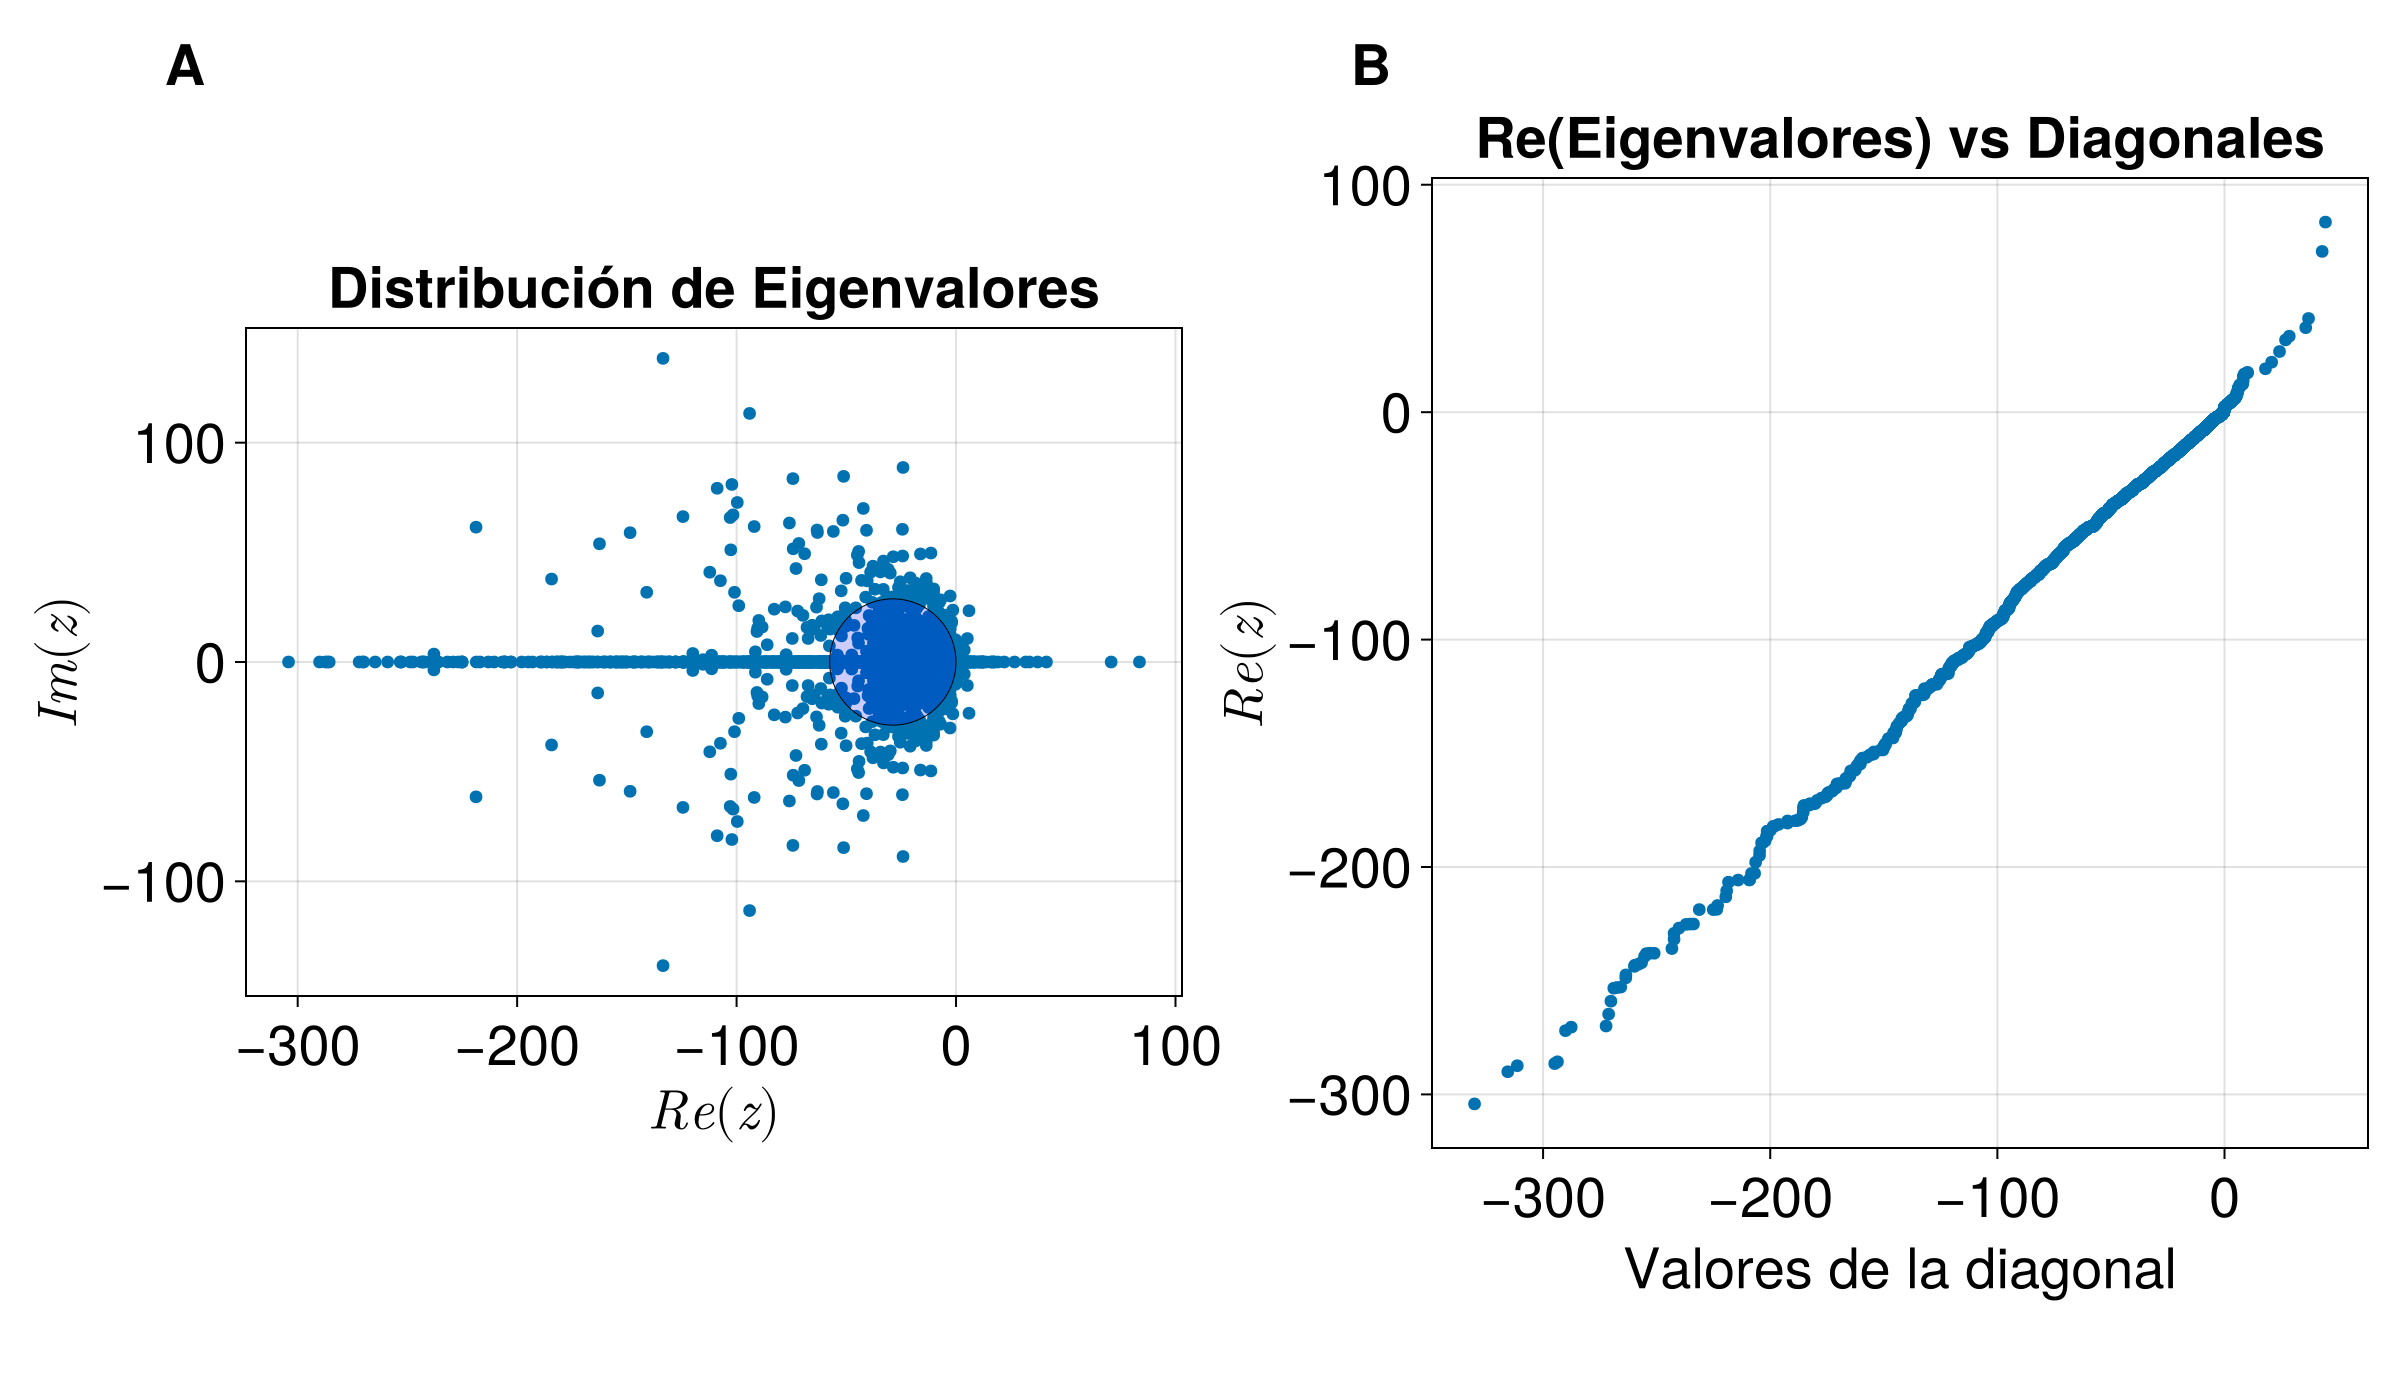
\includegraphics[scale=0.2]{../Imagenes/ReEvs-Diagonales}
	\caption{(\textbf{A}) Distribución de valores propios de 100 jacobianos para el caso $\sigma=0.5$, $p=0.5$. Se agrega una ley circular correspondiente al valor medio de la distribución de diagonales. (\textbf{B}) Relación entre la parte real de los valores propios con las diagonales de los Jacobianos considerados.}
	\label{fig:ReEvs-Diagonales}
\end{figure}

En la distribución de valores propios hay algunas características a analizar: Se ha agregado una ley circular con centro y radio correspondiente al valor medio de su distribución de valores; encierra una gran cantidad de valores propios concentrados en la mancha. Por otro lado se observan valores propios positivos, esto deviene de la discusión que anteriormente se tuvo con respecto de las entradas positivas de las diagonales de los Jacobianos. Hay un porcentaje de éstos que tuvieron valores propios positivos, para evitarlos se debe de considerar en futuras simulaciones un tiempo de integración mayor a 50. En cuanto a la relación entre partes reales de valores propios y elementos de la diagonal de los Jacobianos considerados, existe una relación lineal casi perfecta para el caso particular: $\sigma=0.5$ y $p=0.4$. Sobre todo es interesante ver que incluso existe una relación entre las entradas positivas de las diagonales con los valores propios con parte real positiva, esto ya habla más de la estructura del Jacobiano. En otras distribuciones el ajuste puede ir variando pero en general se sigue esta tendencia entre ambos valores considerados.\\
\\
Para explorar más a profundidad sobre el panorama completo de las simulaciones, se verá la relación entre la media, mediana y moda de las diagonales con respecto de las partes reales de los valores propios de cada uno de los 78 conjuntos de simulaciones; con ello se verá si es que realmente existe una relación lineal entre estas cantidades. Sin embargo, aunque estos sean valores representativos de cada una de las distribuciones, sigue siendo esbozo general.
\begin{figure}[h!]
	\centering
	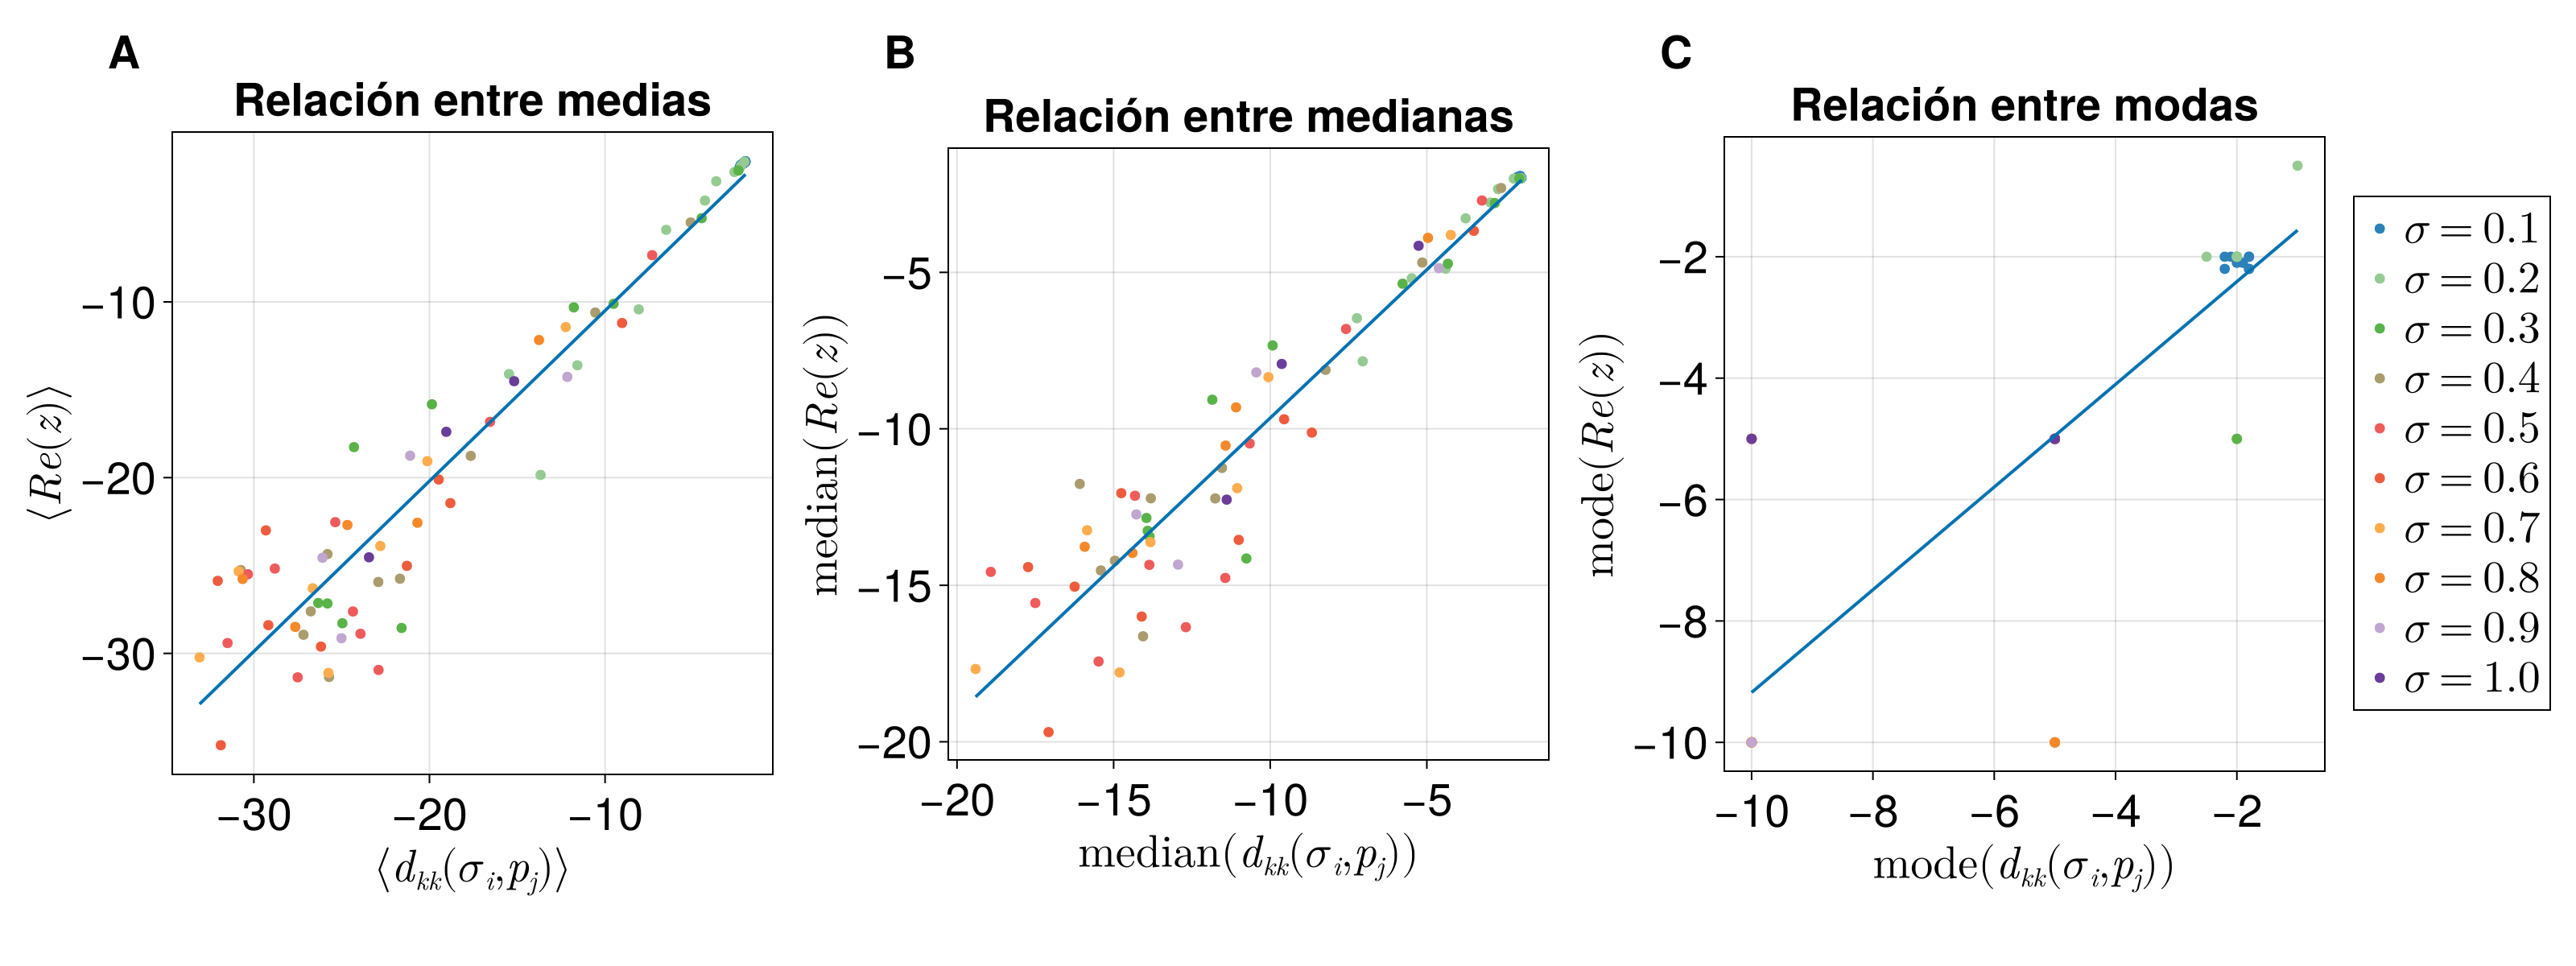
\includegraphics[scale=0.16]{../Imagenes/AjustesLinMeds}
	\caption{(\textbf{A}) Ajuste lineal de la relación entre las medias de las $Re(\overline{\lambda})$ con las medias de las $d_{kk}(\sigma_i,p_j)$ de los Jacobianos del sistema. (\textbf{B}) Ajuste lineal de la relación entre las medianas $Re(\overline{\lambda})$ con las medianas de las $d_{kk}(\sigma_i,p_j))$ de los Jacobianos del sistema. (\textbf{C}) Ajuste lineal de la relación entre las modas de $Re(\overline{\lambda})$ con las modas de las $d_{kk}(\sigma_i,p_j)$ de los Jacobianos del sistema.}
	\label{fig:AjustesLinMeds}
\end{figure}

Estos ajustes lineales al igual que en la Figura (\ref{fig:CorrelacionMvsStd}) es un ajuste general sobre los 78 conjuntos, lo ideal sería realizar un ajuste lineal para cada conjunto $\sigma_i$. Pero de estos gráficos se puede apreciar que para valores cercanos a cero, los 3 casos se ajustan a la recta. Lo que indica que la correlación entre las $d_{kk}(\sigma_i,p_j)$ y las $Re(\overline{\lambda})$ es compartida para toda $\sigma$ con una baja probabilidad de conectividad. Conforme esta $p$ vaya aumentando, entonces la relación lineal se vuelve específica tal y como se mencionó anteriormente. Esta relación esta sugiriendo que la distribución de $Re(\overline{\lambda})$ es semejante a las distribuciones de $d_{kk}(\sigma_i,p_j)$, es decir, ¡de cola pesada y con sesgo negativo! Sin embargo como se mencionó antes: estas medidas aunque son representativas no muestran el panorama completo como en la Figura (\ref{fig:ReEvs-Diagonales} \textbf{B}), pues solo se esta considerando la relación lineal de 3 casos particulares representativos de las distribuciones consideradas. 
\begin{figure}[h!]
	\centering
	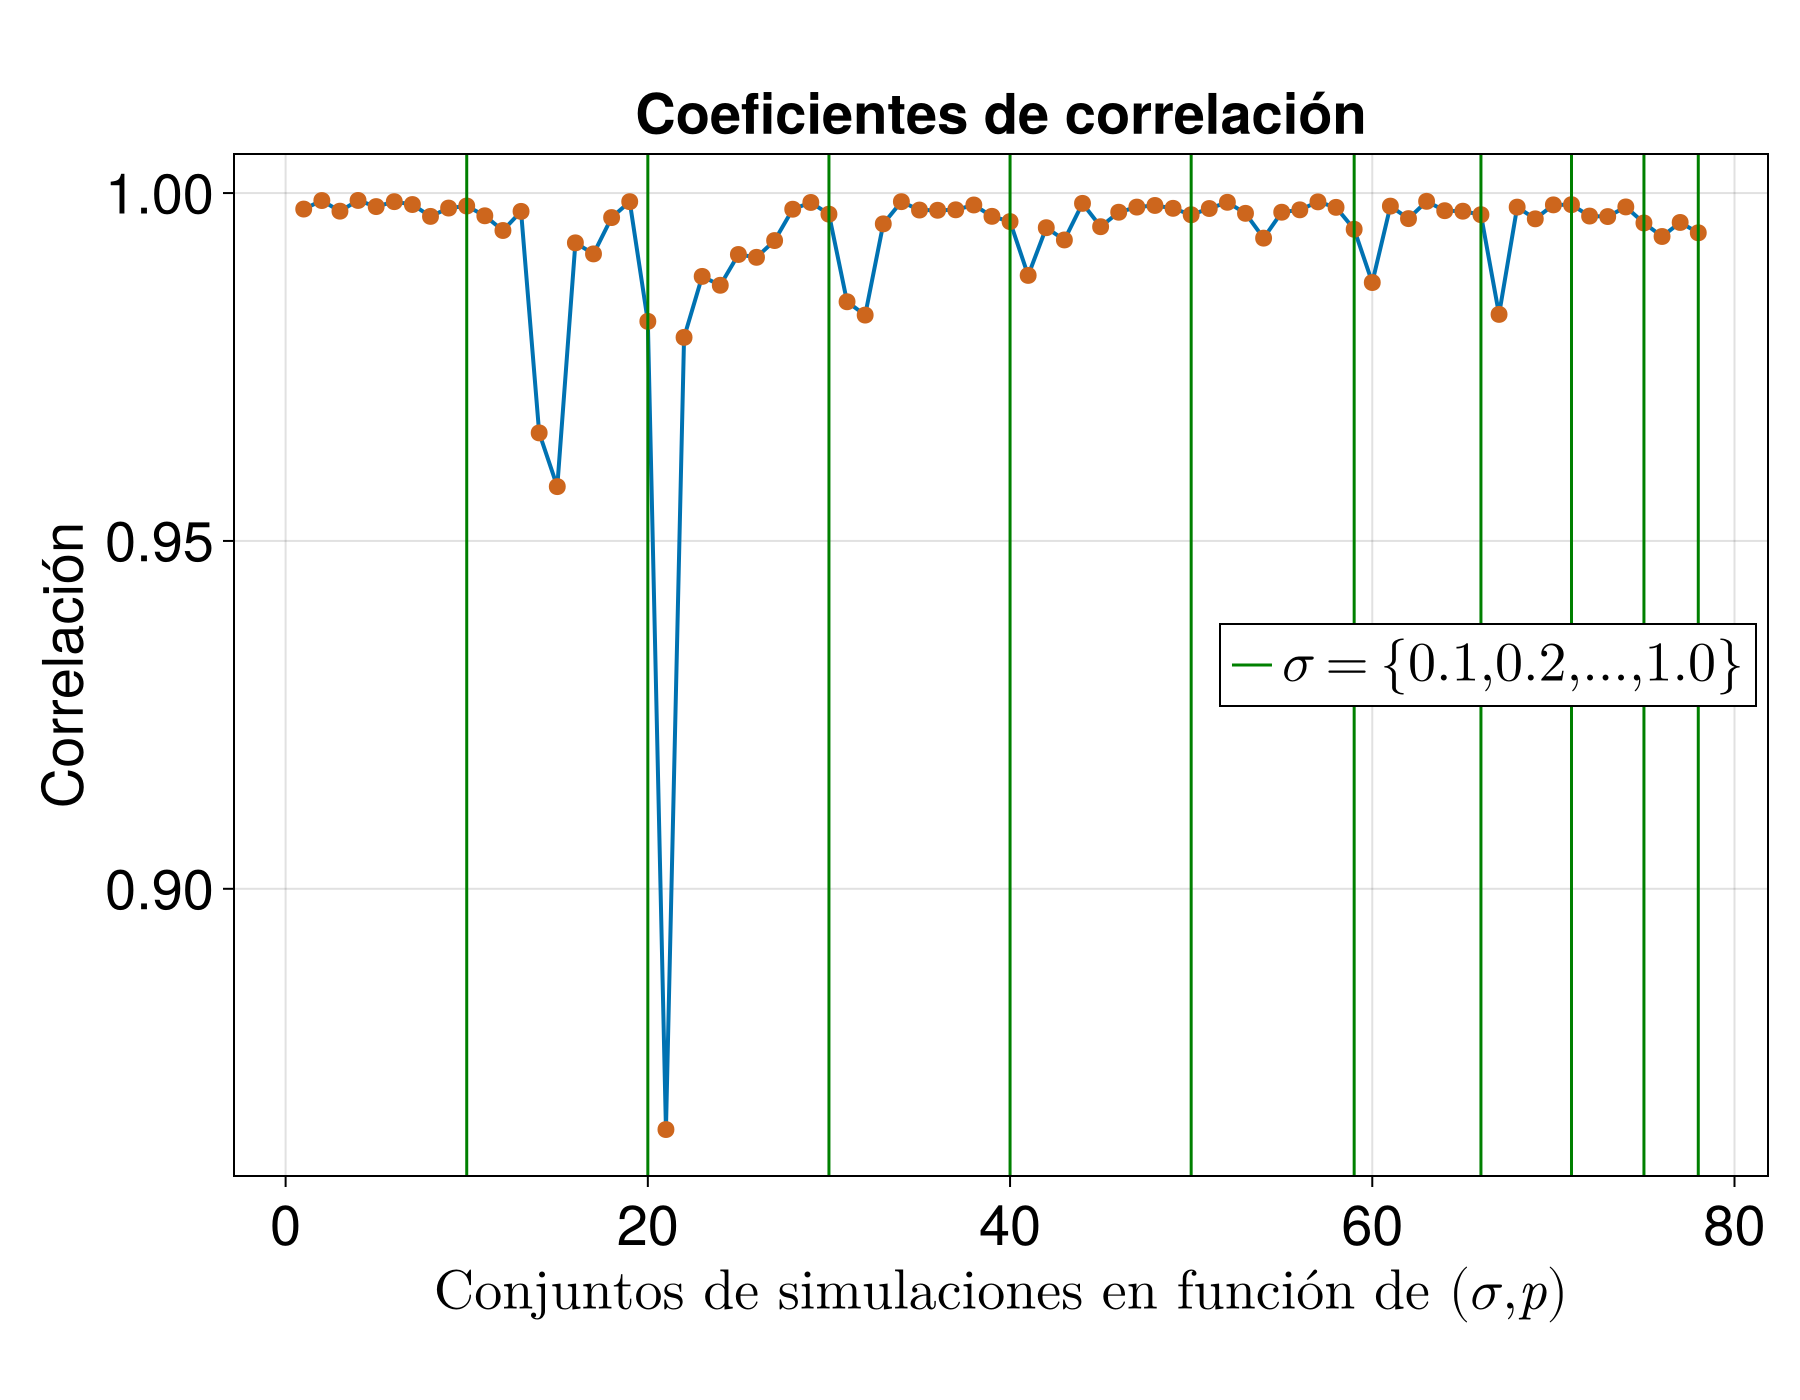
\includegraphics[scale=0.2]{../Imagenes/CoeficientesCorrelacion}
	\caption{Coeficientes de correlación en función de $\sigma$ y $p$. Cada coeficiente corresponde para un conjunto $\sigma_i$ y $p_i$ de simulaciones según la Tabla (\ref{tab:Simulaciones}).}
	\label{fig:CoeficientesCorrelacion}
\end{figure}

Al igual que como se hizo para el coeficiente de variación en la Figura (\ref{fig:CoeficientesVariacion}), se puede armar un mapa de coeficientes de correlación para cada conjunto de simulaciones, de esta manera se podrá ver que tan fuerte o débil es la relación entre $Re(\overline{\lambda})$ y $d_{kk}(\sigma_i,\sigma_j)$. Se puede apreciar que la correlación es sumamente 
\begin{wrapfigure}{r}{0.5 \textwidth} \vspace{-30pt} \begin{center}
		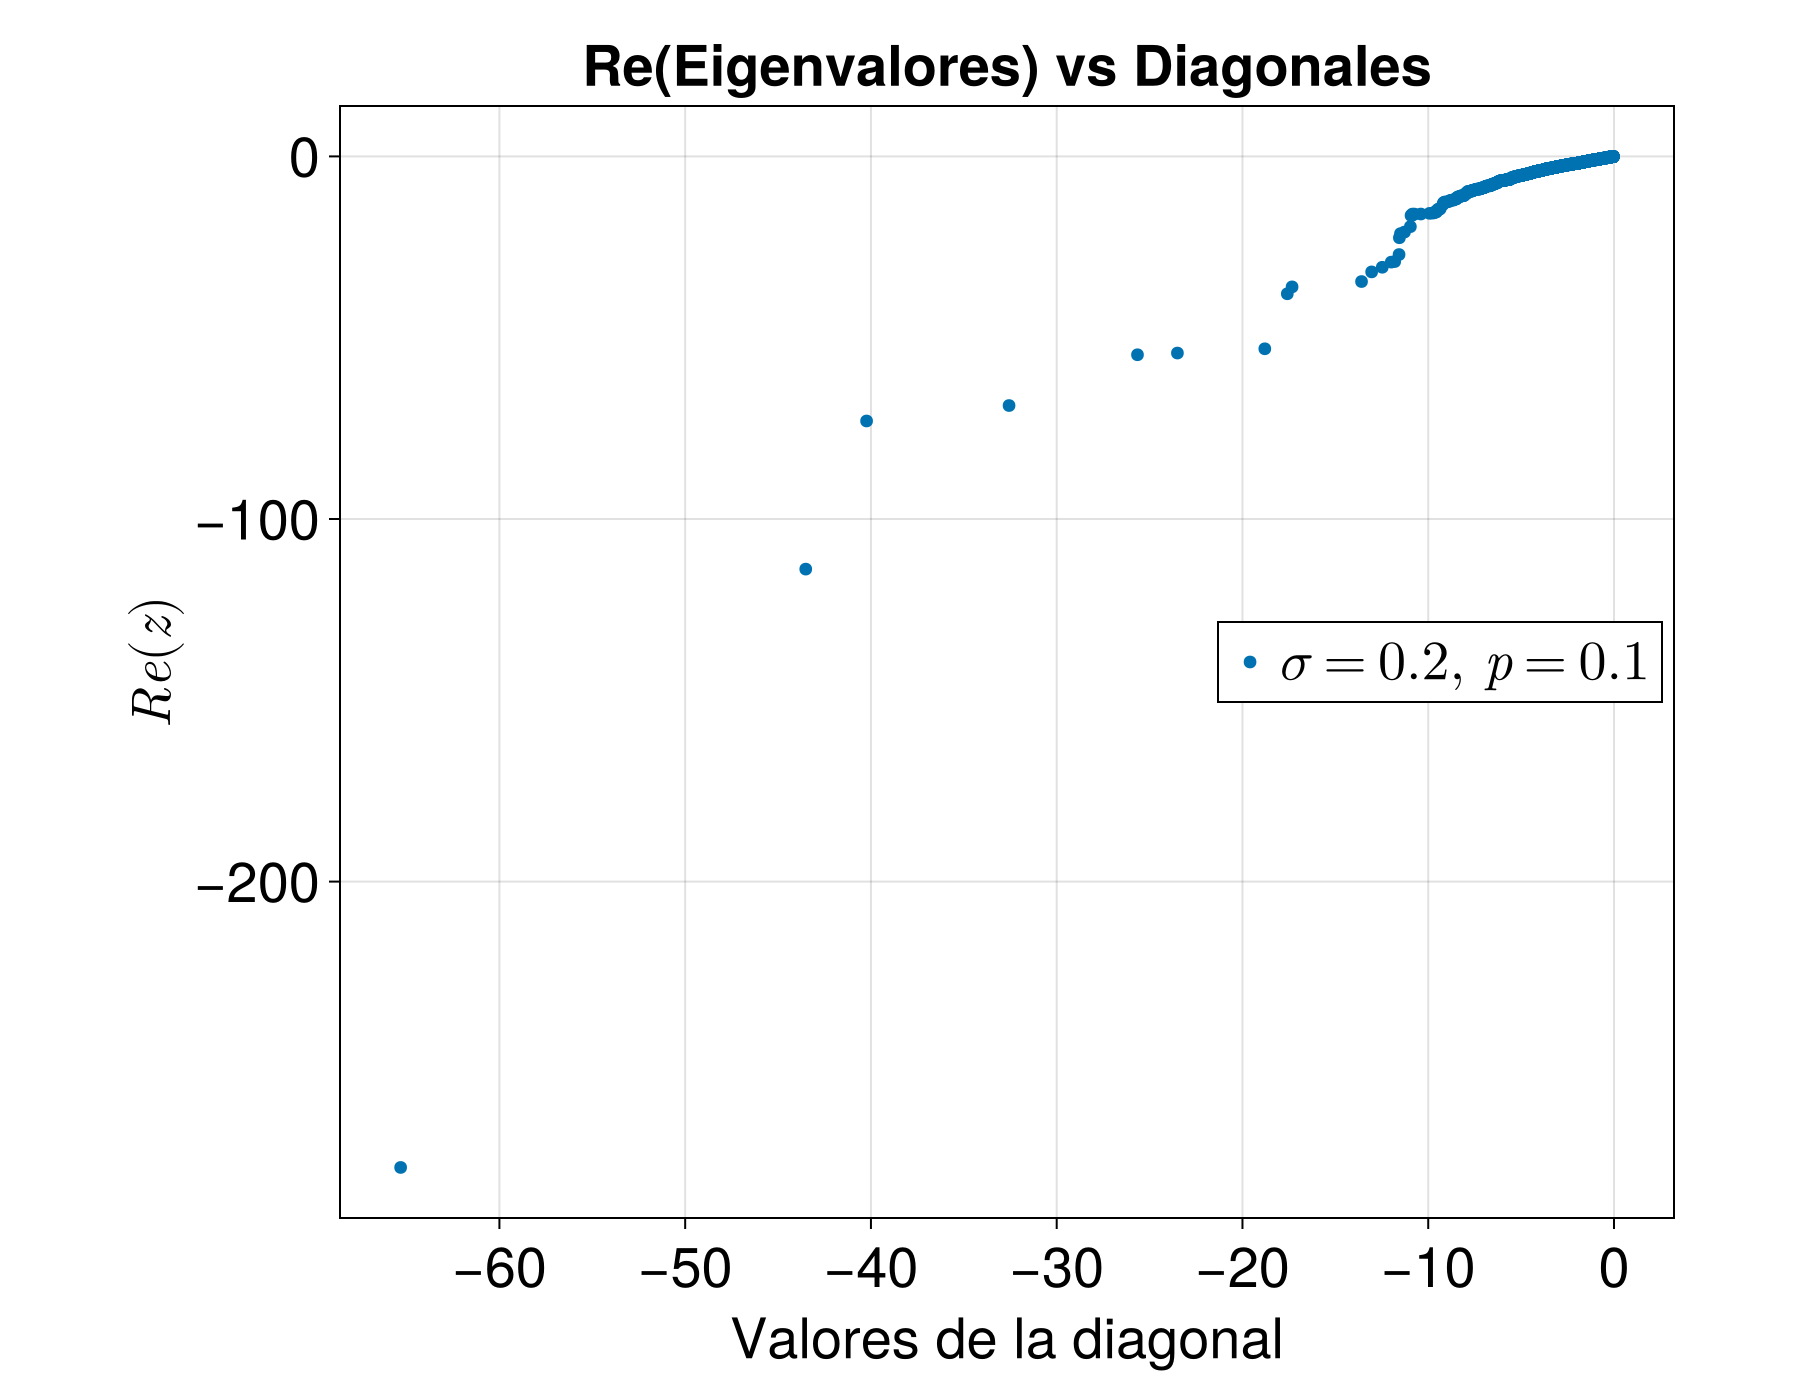
\includegraphics[scale=0.135]{../Imagenes/AnomaliaSim21}
	\end{center}
	\vspace{-20pt} 
	\caption{Anomalía de la simulación 21, caso con $\sigma=0.3$ y $p=0.1$.}
	\vspace{-10pt}
	\label{fig:AnomaliaSim21}
\end{wrapfigure}
fuerte para la gran mayoría de los casos, con valores superiores a $0.98$ lo que indica que las distribuciones de $d_{kk}(\sigma_i,p_j)$ y de $Re(\overline{\lambda})$ no son solamente semejantes sino prácticamente iguales o con muy poca variación. Solamente se tiene una anomalía para el caso $\sigma=0.3$ y $p=0.1$ en el que su coeficiente de correlación es abruptamente más bajo que el resto del conjunto de simulaciones. Viendo como es la relación de este caso particular se observa si hay una tendencia lineal pero hay valores anómalos que no tienen relación entre sí, pues incluso difieren por un orden de magnitud. Sin embargo la tendencia es clara a pesar de las anomalías, el coeficiente es próximo a $0.8654$ y sigue marcando una fuerte correlación entre $Re(\overline{\lambda})$ y $d_{kk}(\sigma_i,p_j)$. Por lo tanto bajo este análisis se puede justificar la propuesta de las $N$ leyes circulares de la Figura (\ref{fig:LeyesCirculares}), los elementos de la diagonal están profundamente relacionados con la distribución de valores propios en el plano complejo. Cada elemento de la diagonal puede ser visto como centro y radio de una ley circular particular y que será capaz de encerrar cierto porcentaje de valores propios que se encuentren a su alcance y dentro de su vecindad.\\
\\
Para concluir esta sección se tienen algunos puntos a abordar; en primer lugar se debe de ver que los casos presentados en esta sección son particulares para $N=50$, habría de definir otros tamaños de matrices para verificar si se siguen los patrones descritos anteriormente. Pero para el mismo caso de $N=50$ se deben de probar más experimentos para otros tipos de tasas de crecimiento y de capacidades de carga, diferentes de $r=2$ y $K=5$ e incluso probar para distribuciones de $r_i$ y de $K_i$ pero claro que al hacerlo se le puede subir uno o varios niveles de complejidad al problema. Al hacer esto se podrá ver si verdaderamente la estructura que se vio en esta sección es universal para cualquier parámetro que se maneje.\\
\\
Los resultados principales de esta sección se enumeran a continuación, las distribuciones de elementos de la diagonal de los Jacobianos asociados al sistema de Lotka-Volterra generalizado siguen una tendencia de distribución de cola pesada con sesgo negativo. Estas distribuciones guardan una relación entre la media y la desviación estándar de modo que para toda $\sigma$, mientras la $p$ aumenta, se ve como la media se recorre hacia valores negativos mientras que la desviación estándar va aumentando. En esta dirección se pudo apreciar que para $\sigma\geq 0.3$ con $p$ bajas: el coeficiente de variación es más grande lo que indica que existe una mayor dispersión en estas distribuciones que en aquellas con $\sigma\geq 0.3$ y $p$ altas, en donde se tienen cada vez más valores en la cola pesada.\\
\\
Las trazas son determinantes para definir la estabilidad del sistema pero no es un criterio absoluto, si se tienen elementos positivos en la diagonal el sistema puede presentar valores propios positivos lo que indica inestabilidad. La misma estructura del Jacobiano del sistema (\ref{eqn:MartizInteracciones}) garantiza los elementos de la diagonal negativos siempre y cuando se evalúe sobre un punto crítico atractor. Las simulaciones nos han confirmado que todo jacobiano evaluado en el atractor produce diagonales con elementos negativos. Por último se ha observado una fuerte correlación entre las $Re(\overline{\lambda})$ y las $d_{kk}(\sigma_i,p_j)$ de los jacobianos del sistema, lo que soporta la justificación de la propuesta de la $N$ leyes circulares que establece que cada uno de los elementos de la diagonal es un centro y radio de una determinada ley circular que encierra cierto porcentaje de valores propios. \\
\\
Además de las propuestas antes mencionadas para investigar otros escenarios del Jacobiano del sistema, una de las cosas que haría falta para completar este trabajo es ver como es la distribución de valores de los elementos fuera de la diagonal de los jacbianos del sistema, ver si son de cola pesada o si tienen algún tipo de sesgo. Observar, caracterizar y ajustar a una distribución conocida para poder crear una receta y así generar estas matrices sin la necesidad de pasar por todo los métodos antes descritos en esta tesis. Un pequeño adelanto de esta idea es comenzando por analizar las curtosis y las modas estadísticas de los elementos fuera de la diagonal de los Jacobianos de uno  de los 78 conjuntos de simulaciones únicamente para saber donde se encuentra el pico de la distribución y determinar si también son de cola pesada
\begin{figure}[h!]
	\centering
	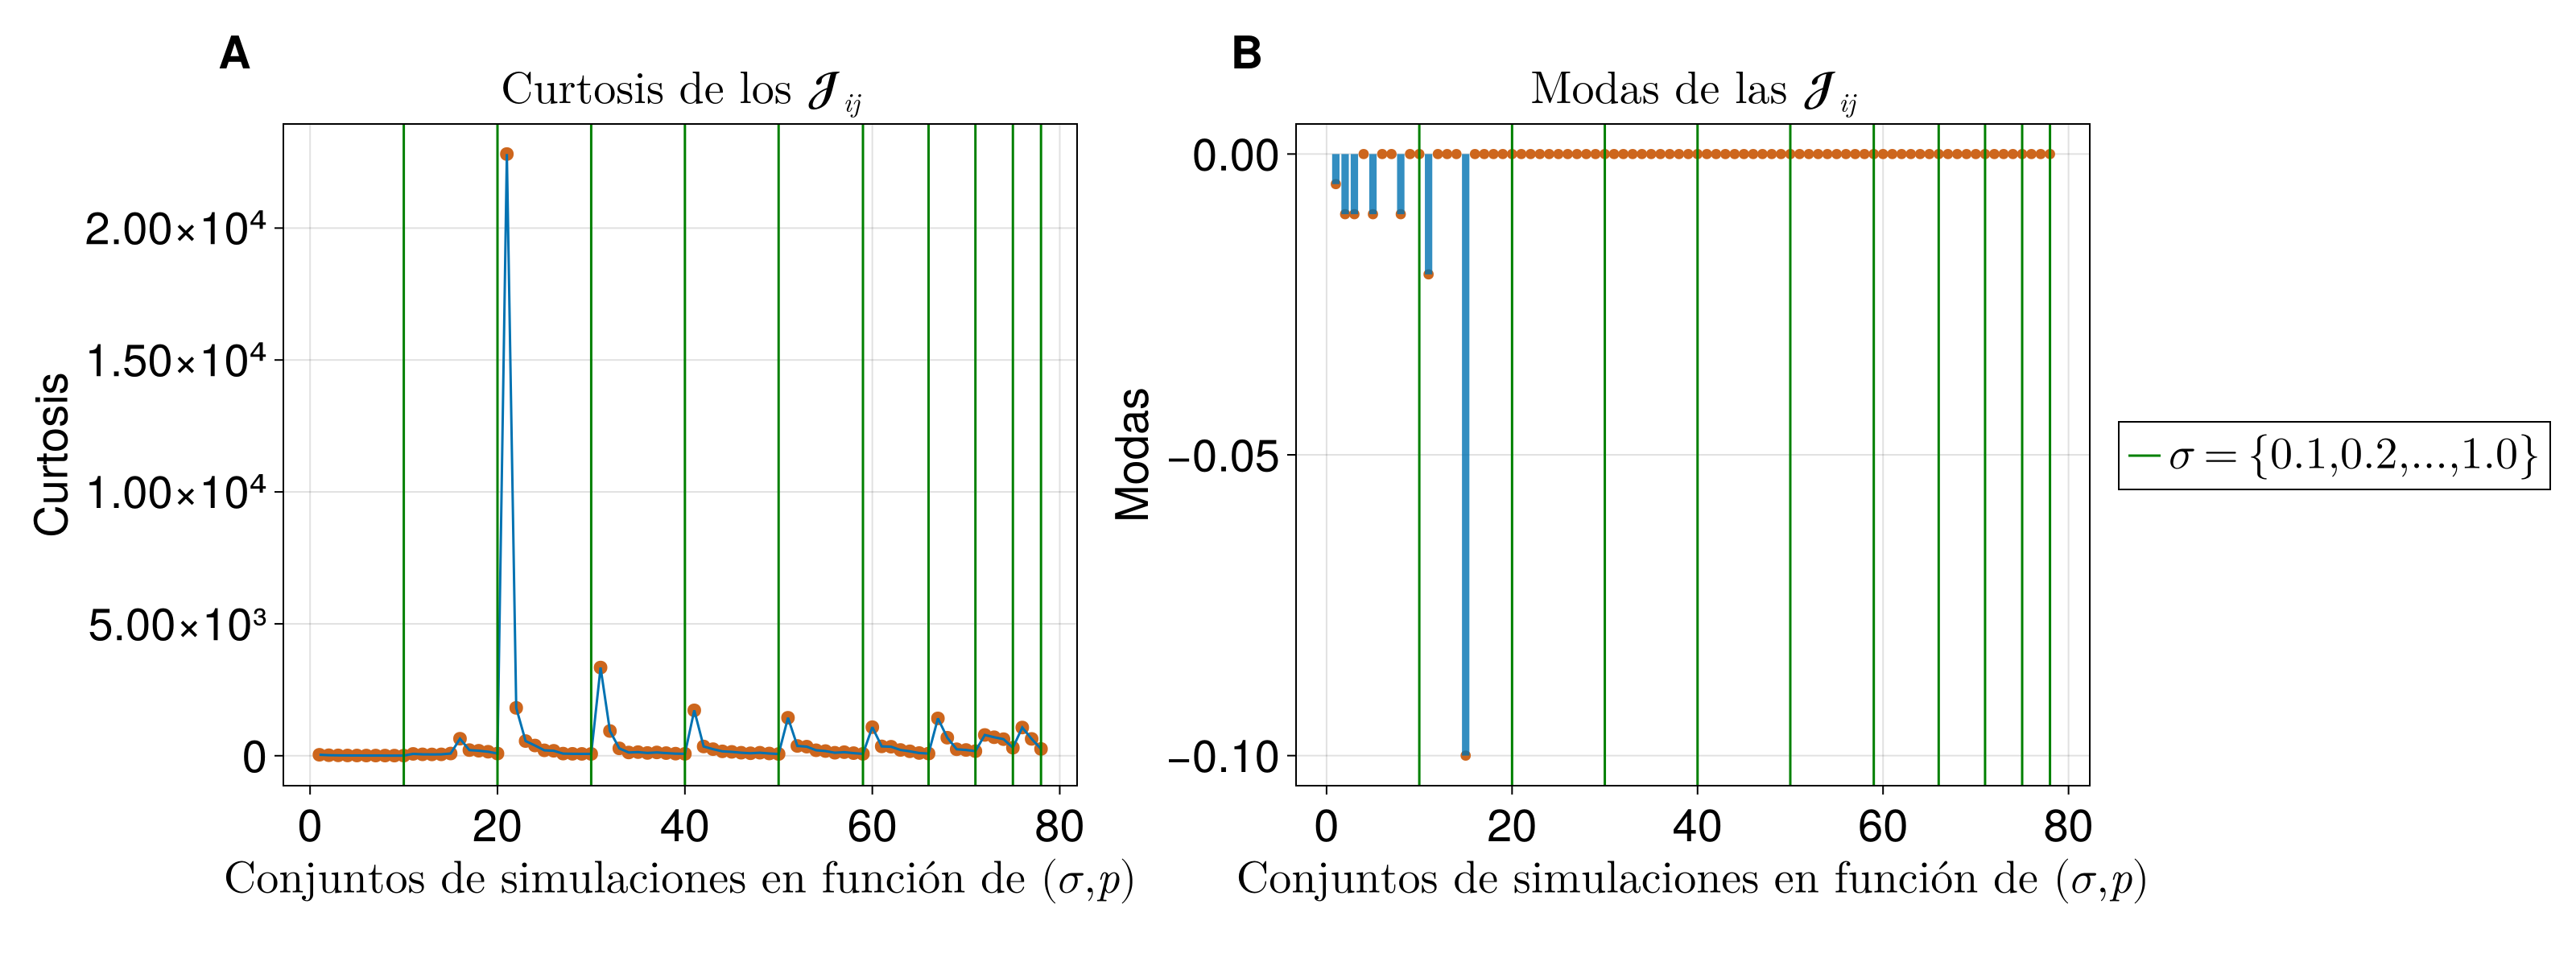
\includegraphics[scale=0.16]{../Imagenes/CurModasJij}
	\caption{(\textbf{A}) Coeficientes de curtosis de los elementos fuera de la diagonal de los Jacobianos del sistema. (\textbf{B}) Modas estadísticas de los elementos fuera de la diagonal de los Jacobianos del sistema.}
	\label{fig:CurModasJij}
\end{figure}

Como se puede observar, son distribuciones muy raras pues en general tienen curtosis muy grandes en particular una que es exageradamente grande con respecto del resto. El valor más frecuente del coeficiente de curtosis para los 78 conjuntos de simulaciones es de 78 lo que sigue siendo muy alto. Además los picos generalmente se encuentran alrededor del cero salvo algunas excepciones. Todo indica que la distribución de valores que conforman los Jacobianos del sistema de Lotka-Volterra generalizado para $N=50$ con $r=2$ y $K=5$ y para cada $\sigma$ y $p$ son sumamente raras: conformados por distribuciones de cola pesada con sesgo negativo para las diagonales, y por distribuciones de cola super pesada centradas en cero para el resto de elementos del Jacobiano. Por lo que realizar la receta de la que se habló anteriormente será una tarea compleja.
\newpage

	
	
	
	
\end{document}